\section{Numerical solutions}
In this section we numerically solve the linear stability problem
corresponding to Eq. \ref{lin_mass}---\ref{lin_energy}. 
We relax the thin-disk, low-frequency and nearly-Keplerian
approximations used in the analytical discussion above, and  
use the full expressions of $\rho$, $\Omega$ and
$\kappa$ given in \S\ref{eqm}. We also restore $\hat{g}_c=1$ to
account for the background radial disk structure.  

%, so that we may consistently consider vertical domains up to
%$z\sim r$.   

We solve the linear problem by expanding the
perturbations in Chebyshev polynomials $T_l$ up to $l=512$
and discretizing the equations on a grid with
$z\in[-\zmax,\zmax]$. At the vertical boundaries we impose a free
surface, 
\begin{align}
  \Delta P \equiv \delta P + \bm{\xi}\cdot\nabla P= 0 \quad \text{at } z=\pm\zmax,
\end{align}
where $\bm{\xi}$ is the Lagrangian displacement. This boundary
condition is convenient for numerical implementation since it conforms
to a standard eigenvalue problem. The above discretization procedure
converts the linear system of differential equations to a set of 
algebraic equations, for which we use matrix routines in the LAPACK
package to solve. 

% mention mode selection -> focus on fundamental corrugation ->
% simulations eventually dominated by them 
% choice of kx is O(10), since nelson observe kxH \sim 30

\subsection{VSI in a locally isothermal, neutrally stratified disk}\label{vertiso_pertiso} 
% disk model is a nearly-vertically
% isothermal disk with $\Gamma=1.011$, $p=-1.5$, $q=-1$,
% $\epsilon=0.1$. 
We first calculate the VSI in a nearly vertcally isothermal, neutrally
straitified disk ($N_z^2\equiv0$) by setting
$\gamma=\Gamma=1.011$ and $\beta=10^{-3}$. Other disk parameters are 
$(p,q,\epsilon)=(-1.5,-1,0.1)$ and the vertical domain is $\zmax =
5\epsilon r$. This setup is similar to that adopted in
\cite{mcnally14}, who calculated the VSI in vertically isothermal
disks subject to isothermal perturbations ($\Gamma=\gamma=1$).  This
allows us to test our numerical code.  

%behaviour as func of kx 

Fig. \ref{iso_eigen_kx} compares the numerically-obtained eigenvalues
for the fundamental mode and that calculated from 
Eq. \ref{sig2_iso} (with $L=1$). There is good agreement for 
$\khat\gtrsim10$. The match worsens for smaller $\khat$ because the 
the low-frequency approximation used to obtain Eq. \ref{sig2_iso} 
is no longer valid, as $|\omega|$ is not small compared to $\Omega_k$
for $\khat\lesssim 10$.  

% This means
% that our analytic results should only be applied to perturbations with
% $\khat\gg 1$, i.e. small radial-lengthscales. 

\begin{figure}
  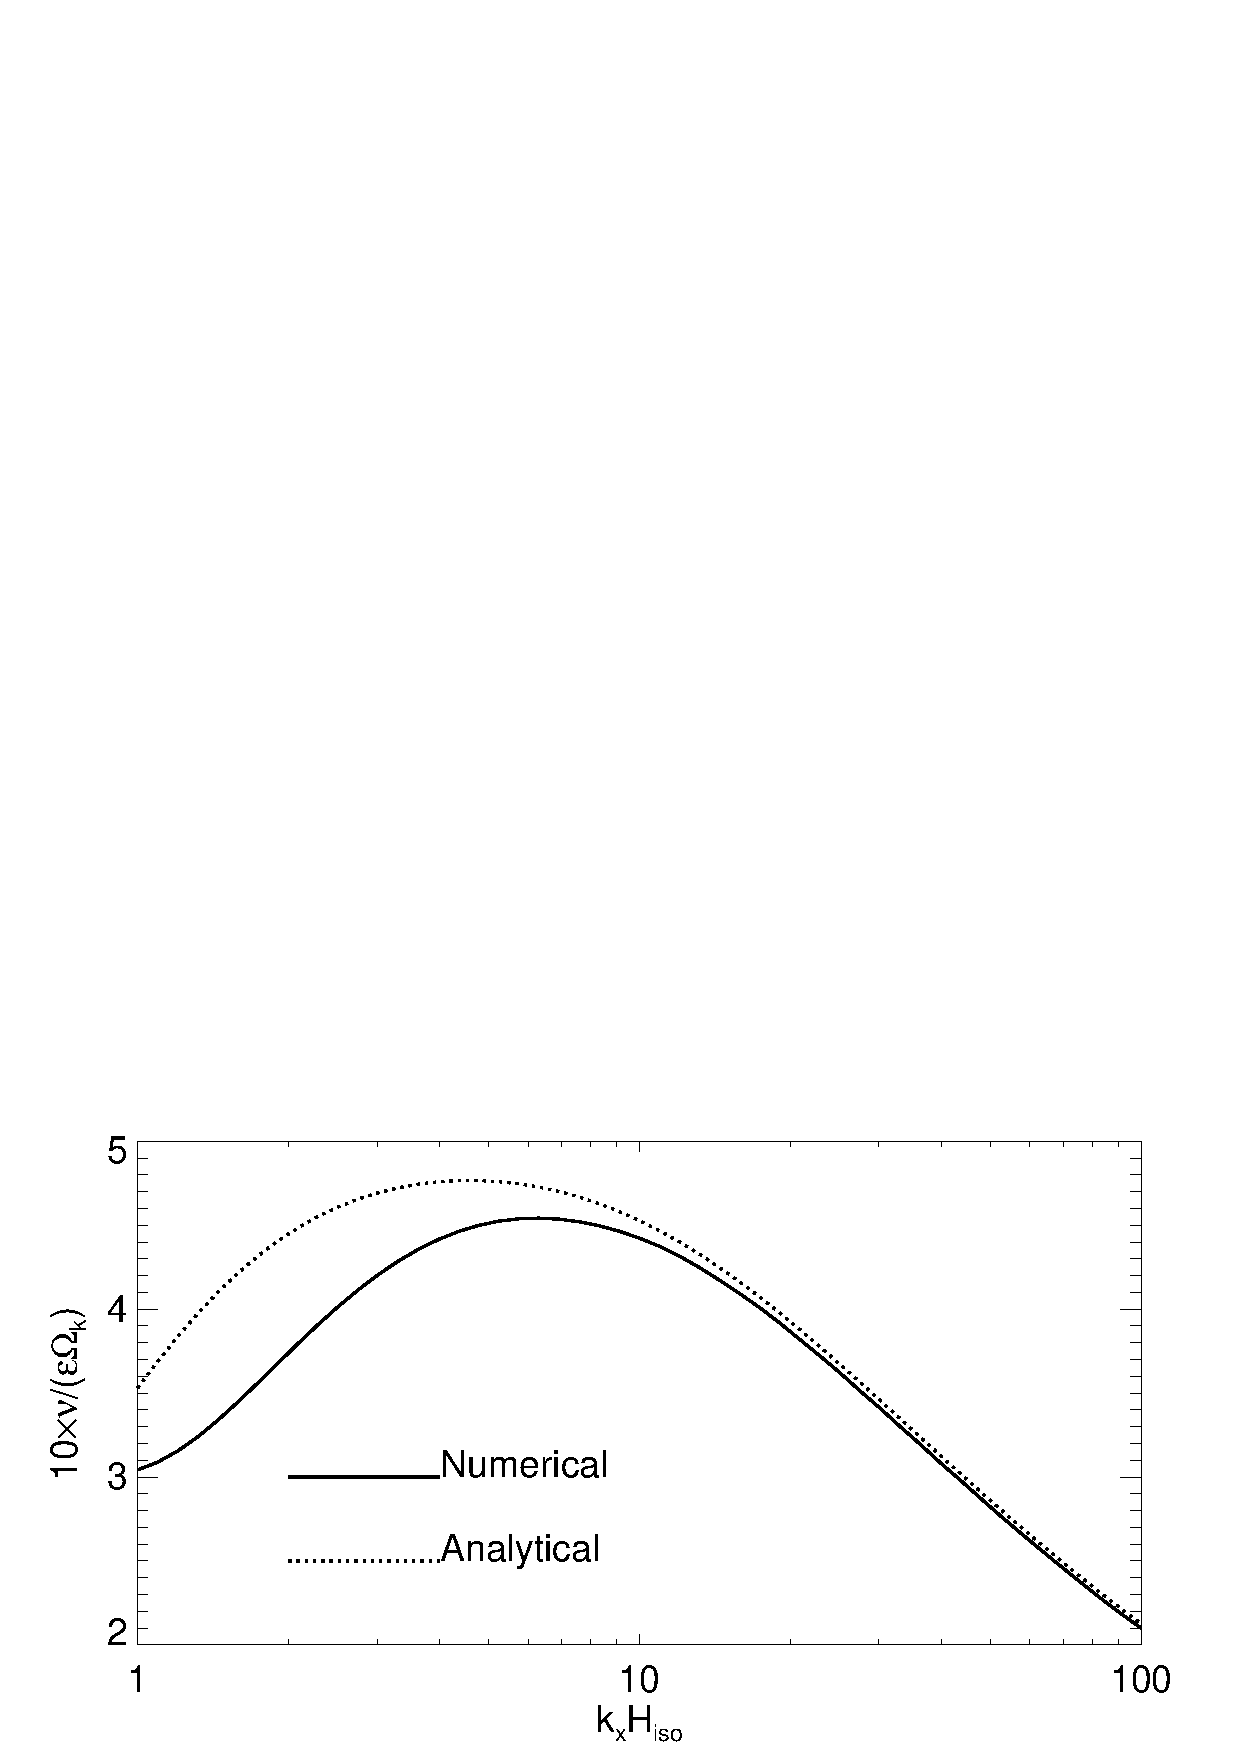
\includegraphics[width=\linewidth,clip=true,trim=0cm 1.75cm 0cm
  0cm]{figures/compare_eigen_imag_iso} 
  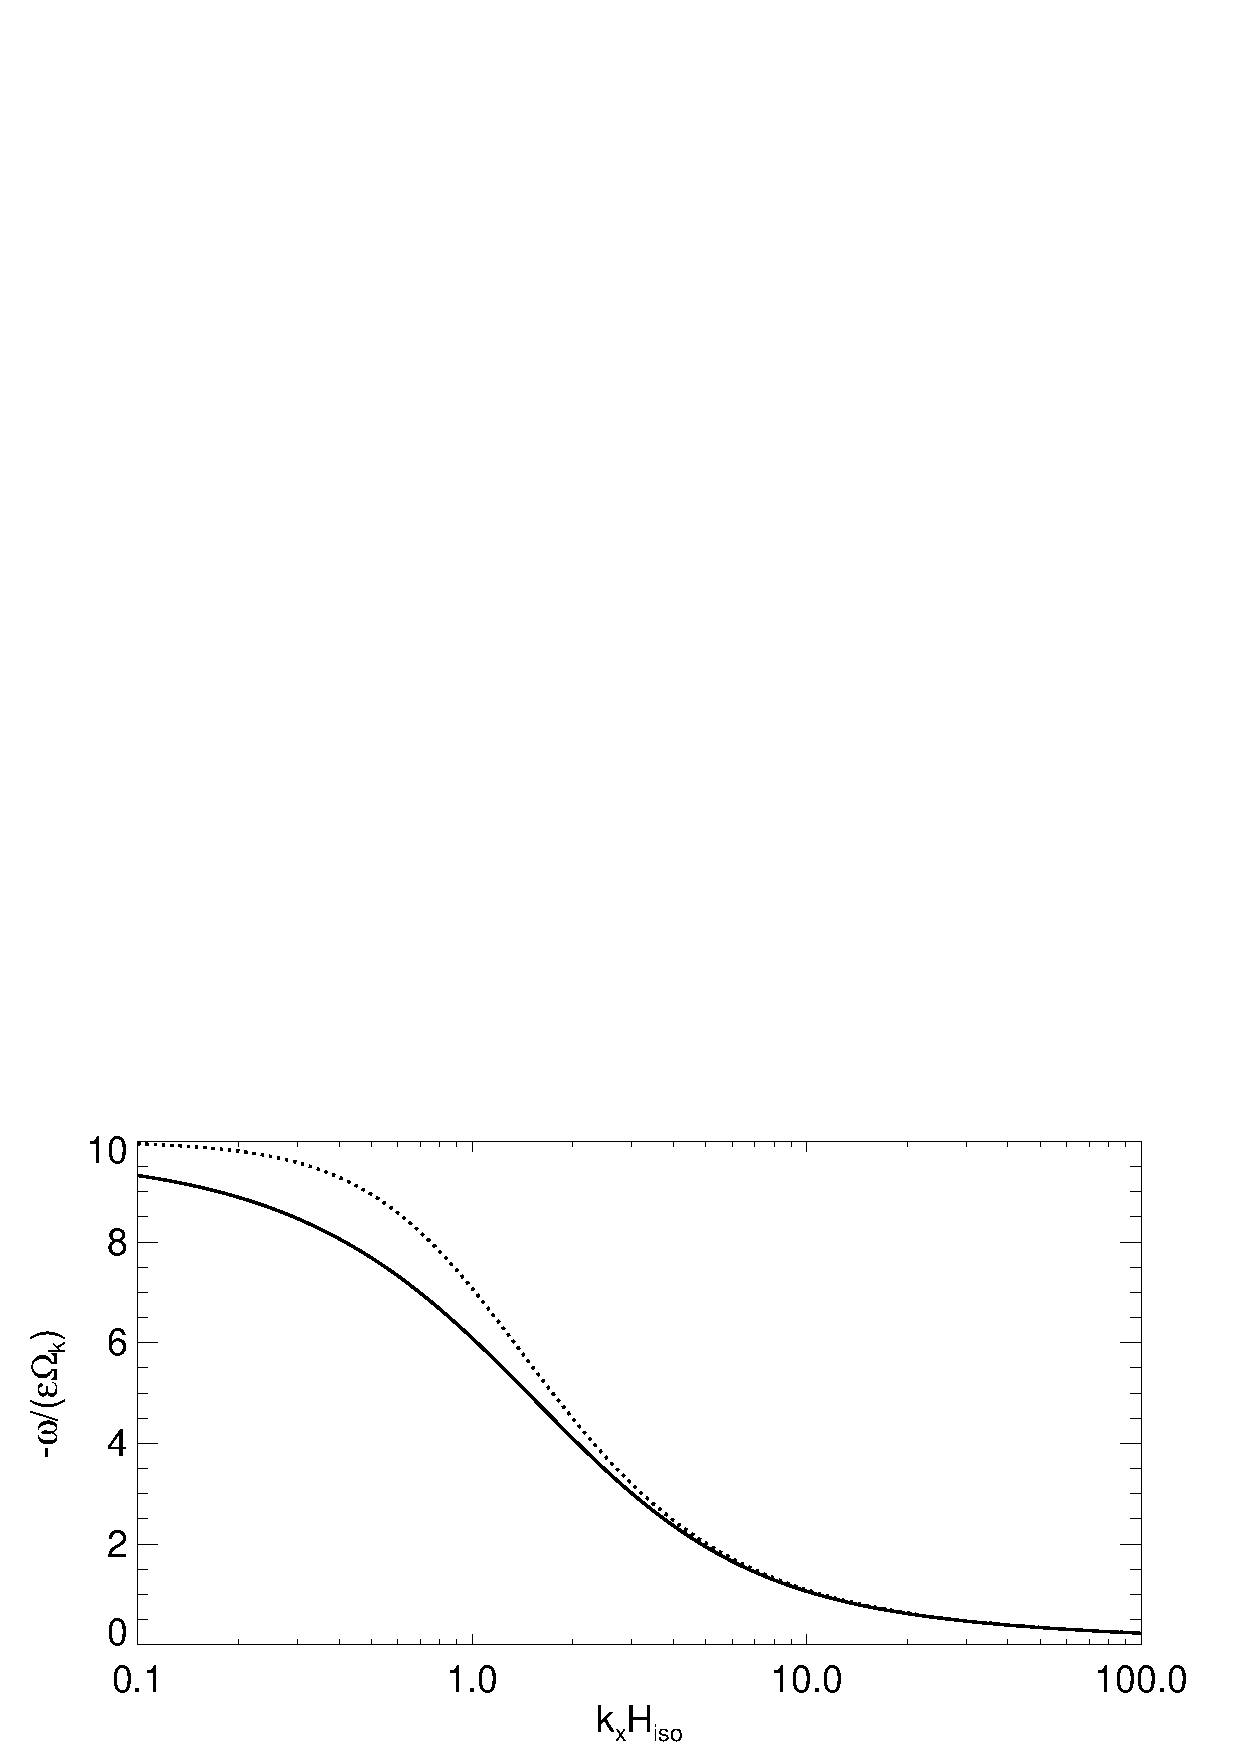
\includegraphics[width=\linewidth,clip=true,trim=0cm 0cm 0cm
  1cm]{figures/compare_eigen_real_iso}
  \caption{Growth rate (top) and real frequency (bottom) of the
    fundamental VSI mode in a disk with $\gamma=\Gamma=1.011$,
    $(p,q,\epsilon)=(-1.5,-1,0.1)$ and
    $\beta=10^{-3}$. The solid (dotted) line is obtained numerically
    (analytically).  
    \label{iso_eigen_kx} 
  }
\end{figure}

Fig. \ref{lowfreq_eigenfunc} compares the fundamental VSI eigenfunction
$W$ for $\khat=1$ and $\khat=20\pi$. The latter value, corresponding
to $k_x= 200\pi/r$, was used by \cite{mcnally14}. We find $W$ is
similar for all $\khat\gtrsim10$ and is proportional to $z$, as
expected for the fundamental mode according to explicit solutions
developed in \S\ref{iso_poly}.  

However, for $\khat\lesssim 10$, e.g. $\khat=1$ in 
Fig. \ref{lowfreq_eigenfunc}, the perturbation magnitude near the
boundaries begin to dominate. For even smaller $\khat\lesssim 1$ (not
shown) we find the perturbation is almost entirely concentrated at the
boundaries. Our radially-local approximation is likely invalid for 
these small wavenumber perturbations and we do not consider such modes
further.      

\begin{figure}
  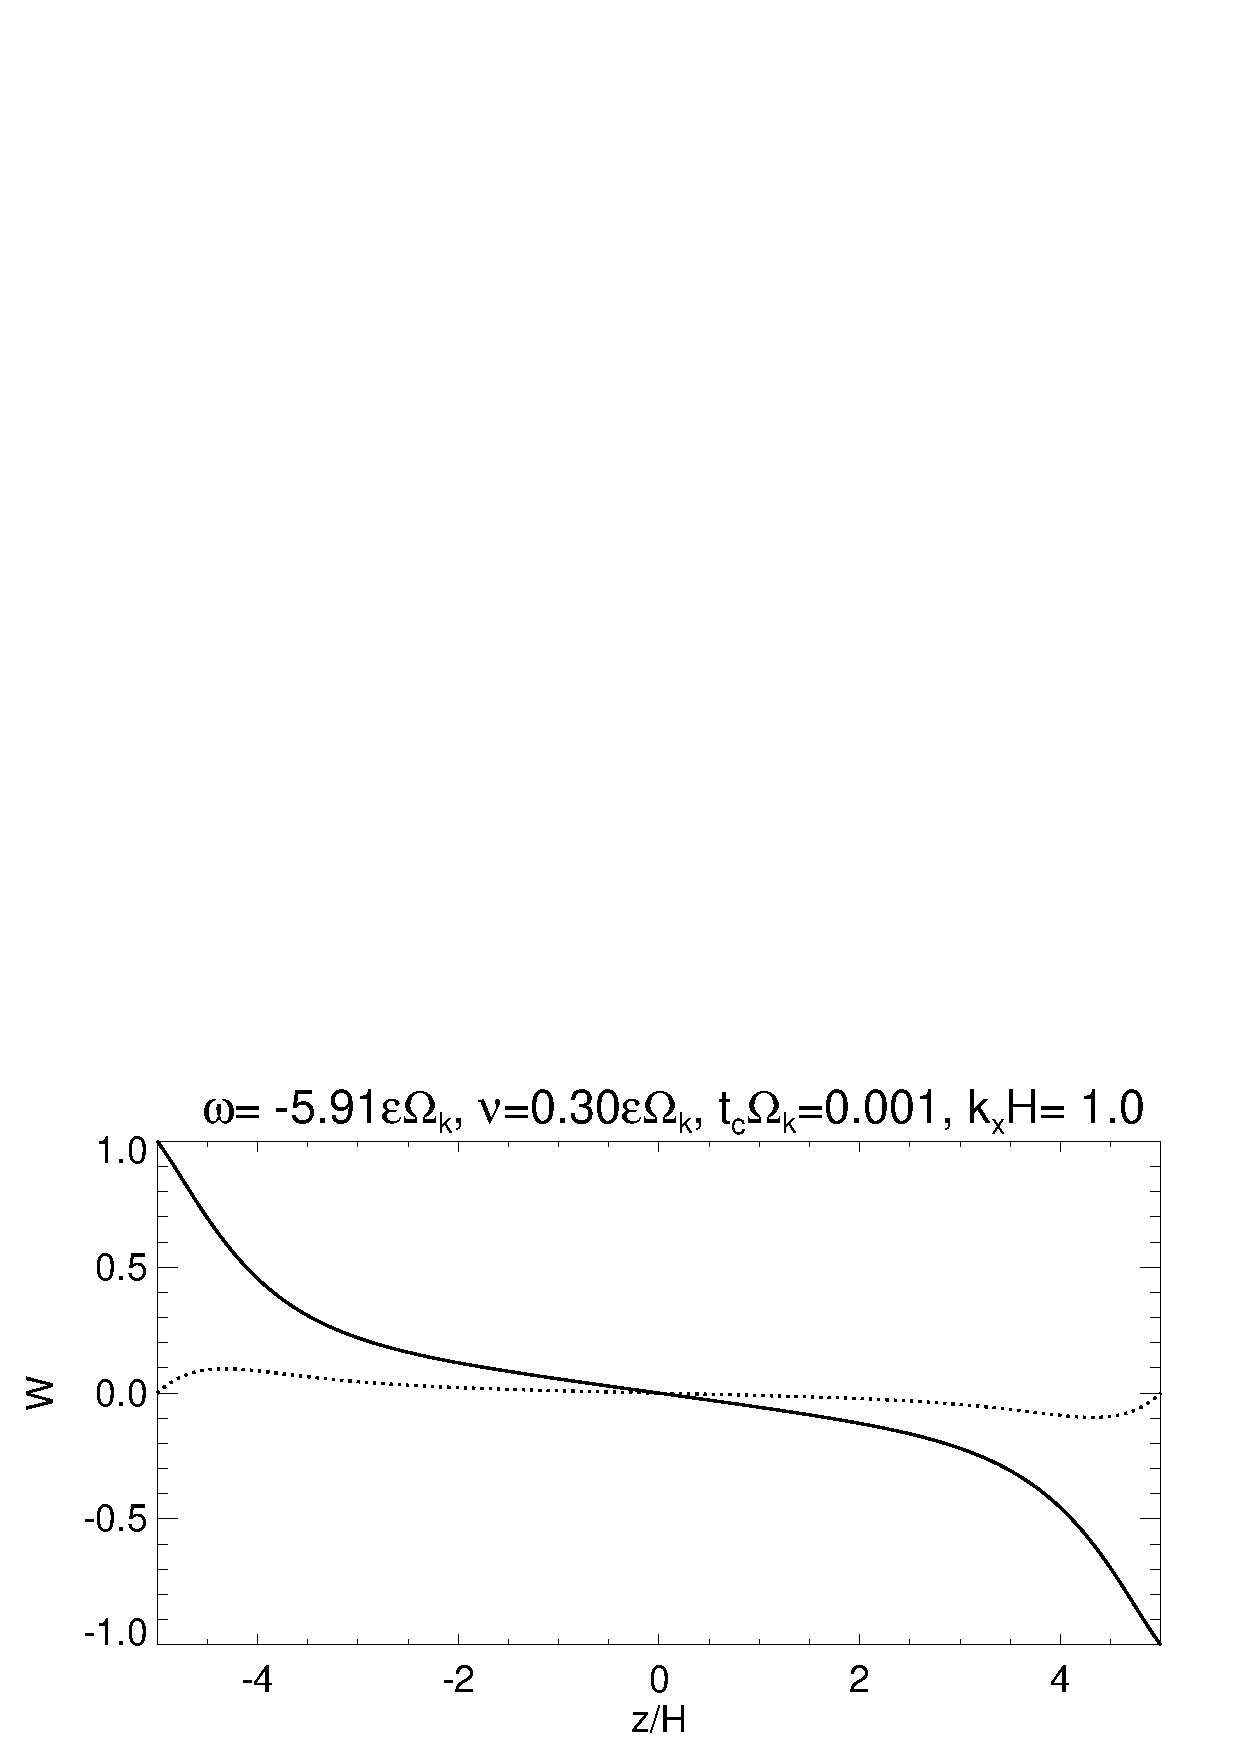
\includegraphics[width=\linewidth,clip=true,trim=0cm 1.75cm 0cm
  0cm]{figures/eigenvector_iso_kx1} 
  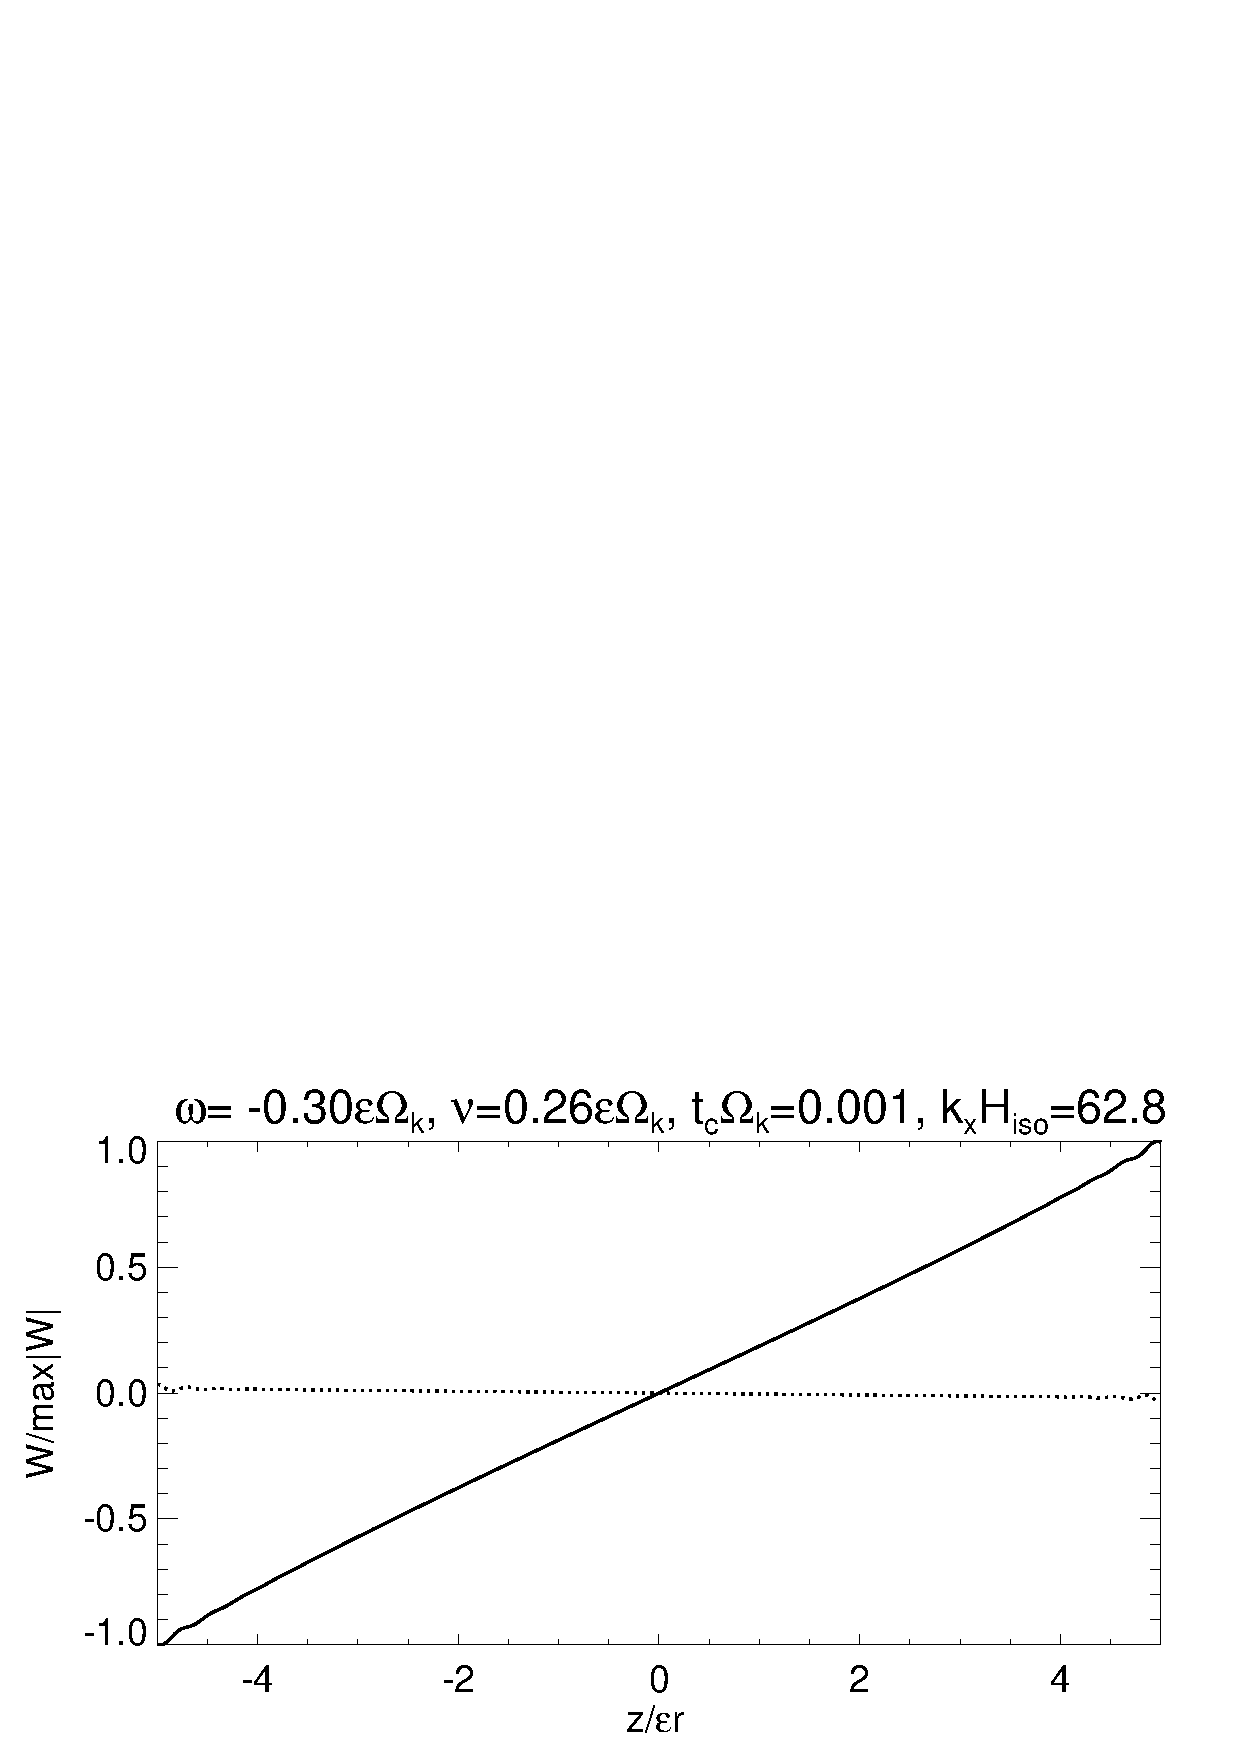
\includegraphics[width=\linewidth]{figures/eigenvector_iso_kx60}
  \caption{Eigenfunction of the fundamental VSI for perturbation
    wavenumber $\khat=1$ (top) and $\khat=20\pi$ (bottom). The real 
    (imaginary) parts of $W$ are plotted as solid (dotted) lines. 
    \label{lowfreq_eigenfunc}
  }
\end{figure}

In Fig. \ref{lowfreq_eigen} we plot the eigenvalues 
$\sigma = \omega + \ii\nu$ found for $\khat=20\pi$. This plot is
similar to Fig. 3 in \cite{mcnally14}. The fundamental
VSI mode, with one node in $W$, has the smallest $|\sigma|$. The
eigenvalue calculated from Eq. \ref{sig2_iso} with $L=1$ and the 
numerically-obtained value are  
\begin{align*}
  (\omega,\nu) = (-0.3053,0.2606)\epsilon\Omega_k &\quad \text{(from
    Eq. \ref{sig2_iso})},\\
  (\omega,\nu) = (-0.3010,0.2575) \epsilon \Omega_k &\quad \text{(numerical)}.
\end{align*}
This agreement is surpsingly good given the number of approximations
used to obtain Eq. \ref{sig2_iso}, which also imposes a different
boundary condition to that in the numerical calculation. These values
are also close to that found by \cite{mcnally14}. The eigenfrequency
is not sensitive to the vertical boundary condition because the
expression for $\sigma$, given by Eq. \ref{integral_relation1},
involve integrands with $\rho$ as the   weight function, which rapidly
decays away from the midplane. 

\begin{figure}
  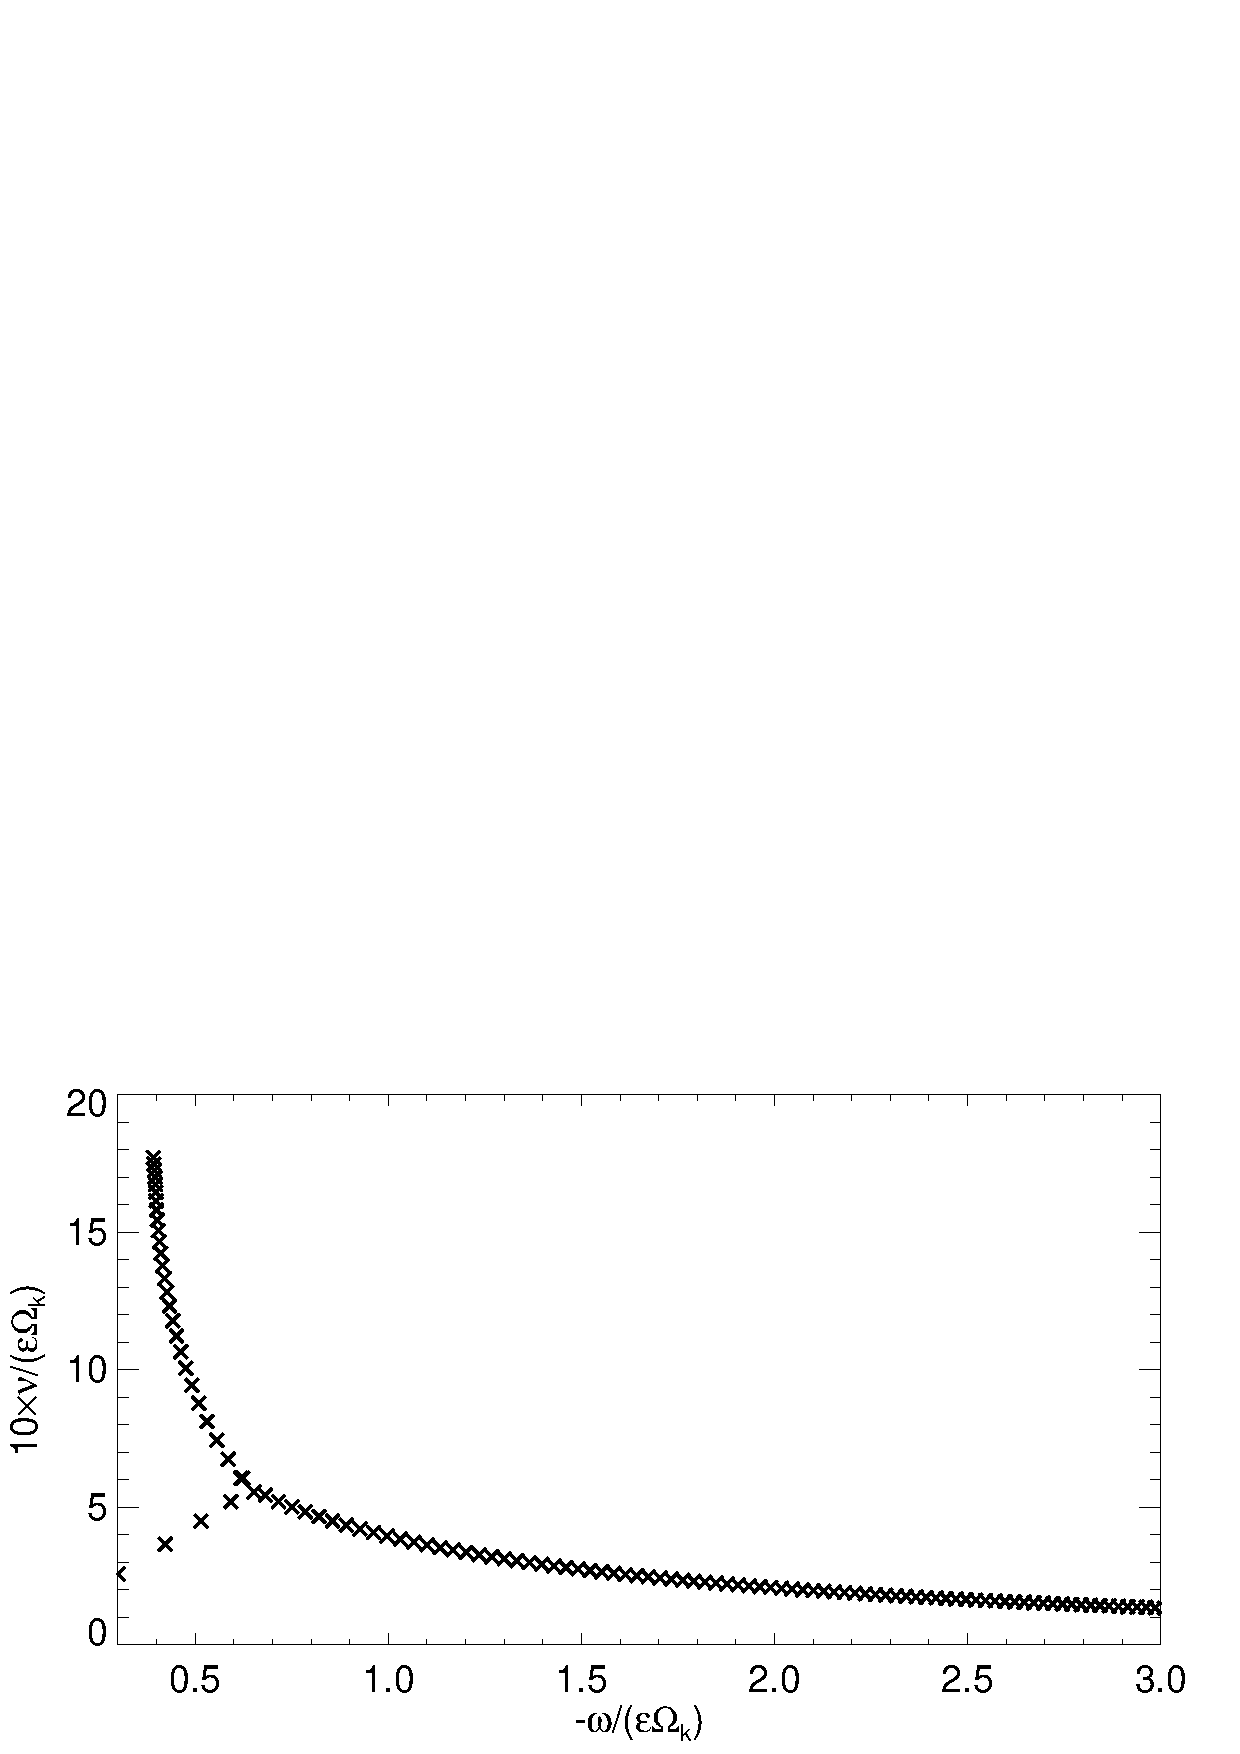
\includegraphics[width=\linewidth]{figures/eigenvalues_iso}
  \caption{Eigenvalues of perturbations with wavenumber $\khat=20\pi$
    in a neutrally-stratified, nearly-vertically isothermal disk
    ($\gamma=\Gamma=1.011$) with $(p,q,\epsilon)=(-1.5,-1,0.1)$ and
    $\beta=10^{-3}$. \label{lowfreq_eigen} 
  }
\end{figure}

\subsection{Effect of thermal relaxation}
We now consider stably stratified disks ($\gamma > \Gamma$) with
thermal relaxation $\beta\in[10^{-3},1]$. Here we use a slightly  
different disk model with $\epsilon=0.05$ and $\gamma=1.4$, as 
adopted in simulations performed by \cite{nelson13}. Other parameters 
are unchanged from the previous section.  

Fig. \ref{bcrit_compare1} shows the growth rate $\nu$ of the
fundamental VSI mode as a function of $\beta$ for $\khat=30$. This is
approximately the perturbation wavenumber observed in the fiducial
numerical simulation of \cite{nelson13}. We also plot the growth rates
obtained by numerically solving the dispersion relation 
Eq. \ref{relax_disp} and the upper limit to 
the thermal relaxation timescale $\beta_\mathrm{crit}$ given by
Eq. \ref{iso_vsi_cond}. For the present disk parameters
$\beta_\mathrm{crit}=0.125$. 

We find good agreement between the numerical and analytical growth
rates, as well as the critical relaxation timescale. Growth rates are
insensitive to $\beta$ for $\beta\lesssim 0.05$, beyond which growth
rates rapidly decrease. For this disk model, \citeauthor{nelson13}
found a thermal relaxation timescale of $\beta\gtrsim 0.6$ stabilized
the VSI in non-linear hydrodynamic simulations. This is consistent
with our results.   

%implications for nonlinear sims?

 \begin{figure}
   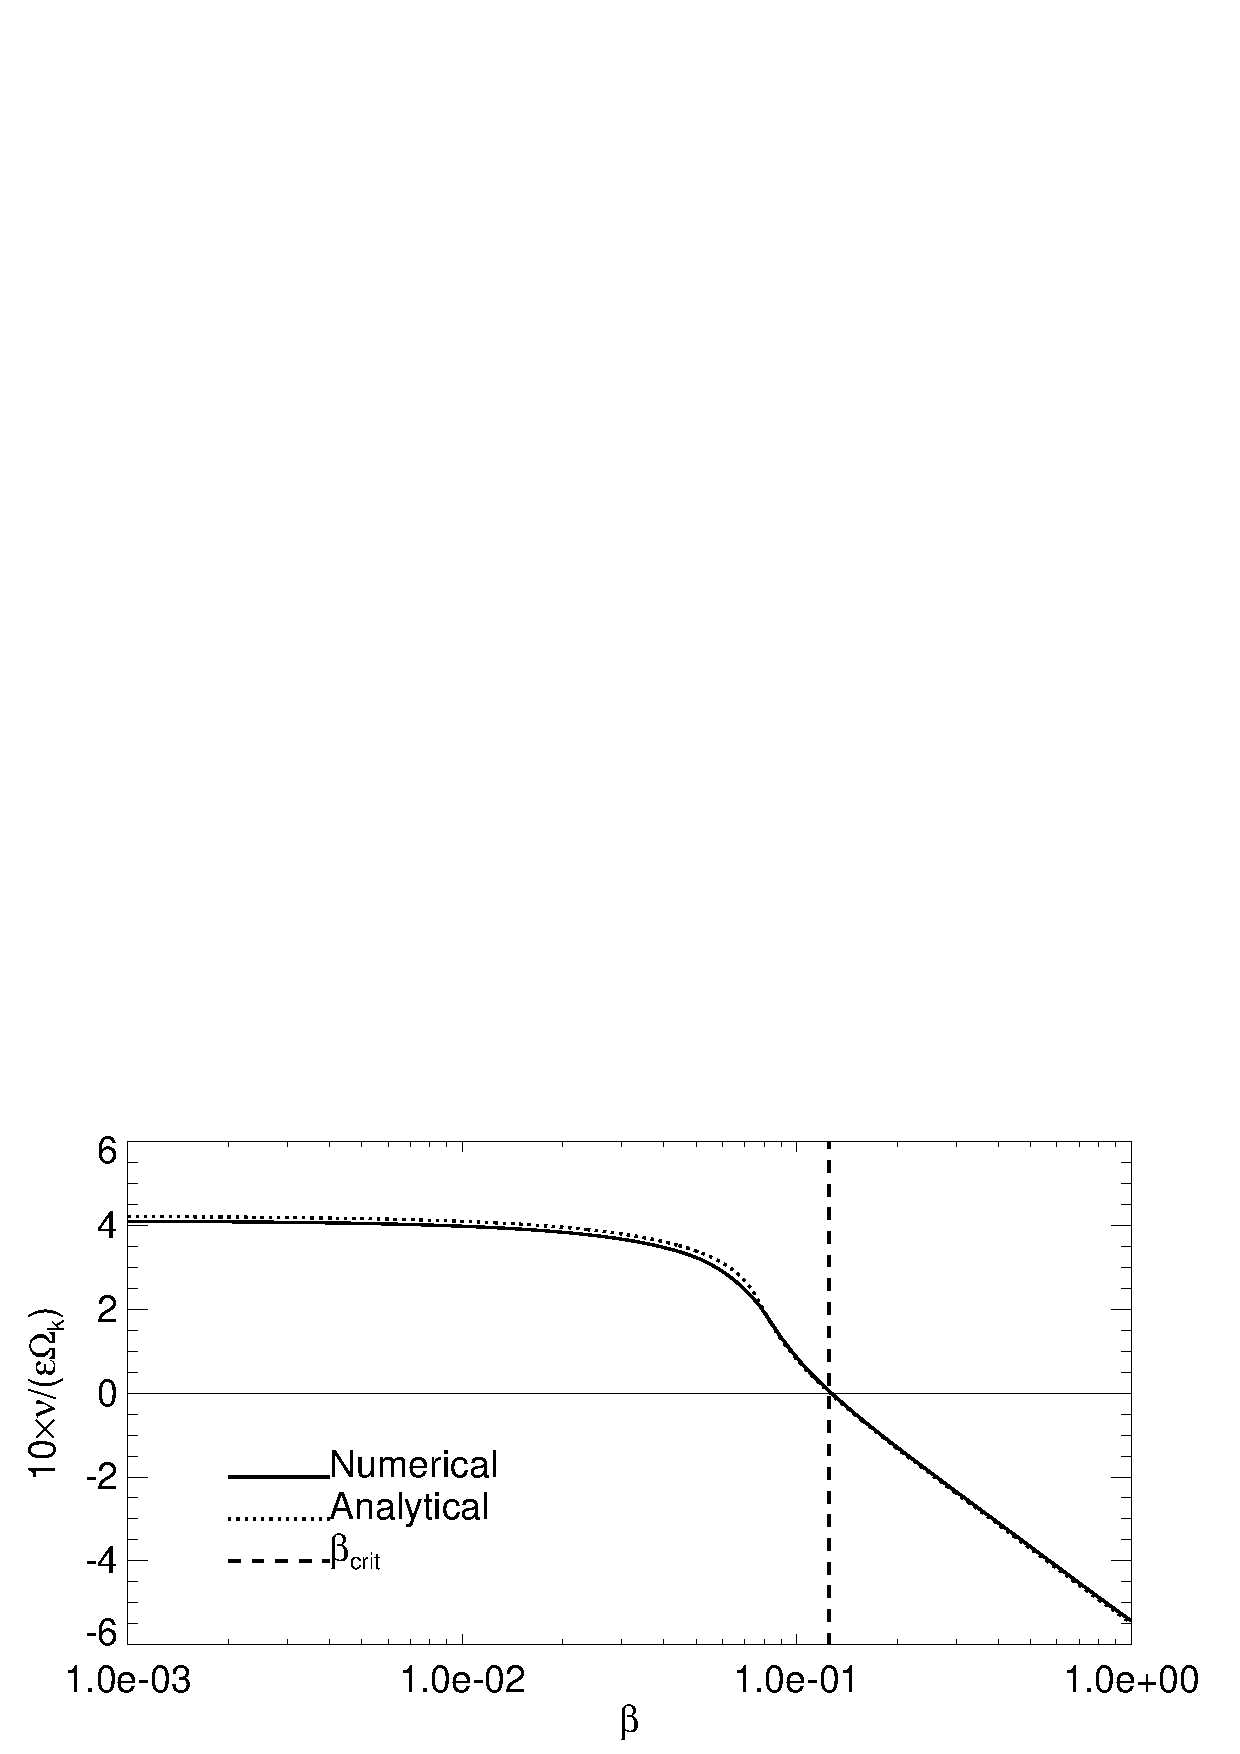
\includegraphics[width=\linewidth]{figures/bcrit_compare} 
   \caption{Growth rate of the fundamental VSI mode with $\khat=30$ as
     a function of the thermal relaxation timescale $\beta$. The disk
     parameters are $\Gamma=1.011$, $\gamma=1.4$, and 
     $(p,q,\epsilon)=(-1.5,-1,0.05)$. The numerical (analytical) growth
     rates are show as solid (dotted) lines, while the vertical line
     is the maximum thermal timescale $\beta_\mathrm{crit}$ for the
     fundamental mode according to Eq. \ref{iso_vsi_cond}. 
     \label{bcrit_compare1}}   
 \end{figure} 

% Fig. \ref{relax_growth_num} shows the growth rates of the fundamental  
% mode as a function of $\khat$. This plot is largely consistent with  
% Fig. \ref{relax_disp_fig} except for $\khat\lesssim 1$
% where the low-frequency approximation fails. (In any case, the local model not valid
% for $\khat\ll1$.) For $\khat\gtrsim 10$ introducing thermal
% relaxation rapidly stabilizes the fundamental mode. 


% Fig. \ref{relax_growth_num} also confirms our analytical discussion that
% introducing a small but finite cooling time stabilizes the fundamental
% VSI, but there is a preferable wavenumber that maximizes this effect (\S\ref{relax_pert}).
% This occurs at $\khat= O(10)$ for the current disk model. 

% \begin{figure}
%    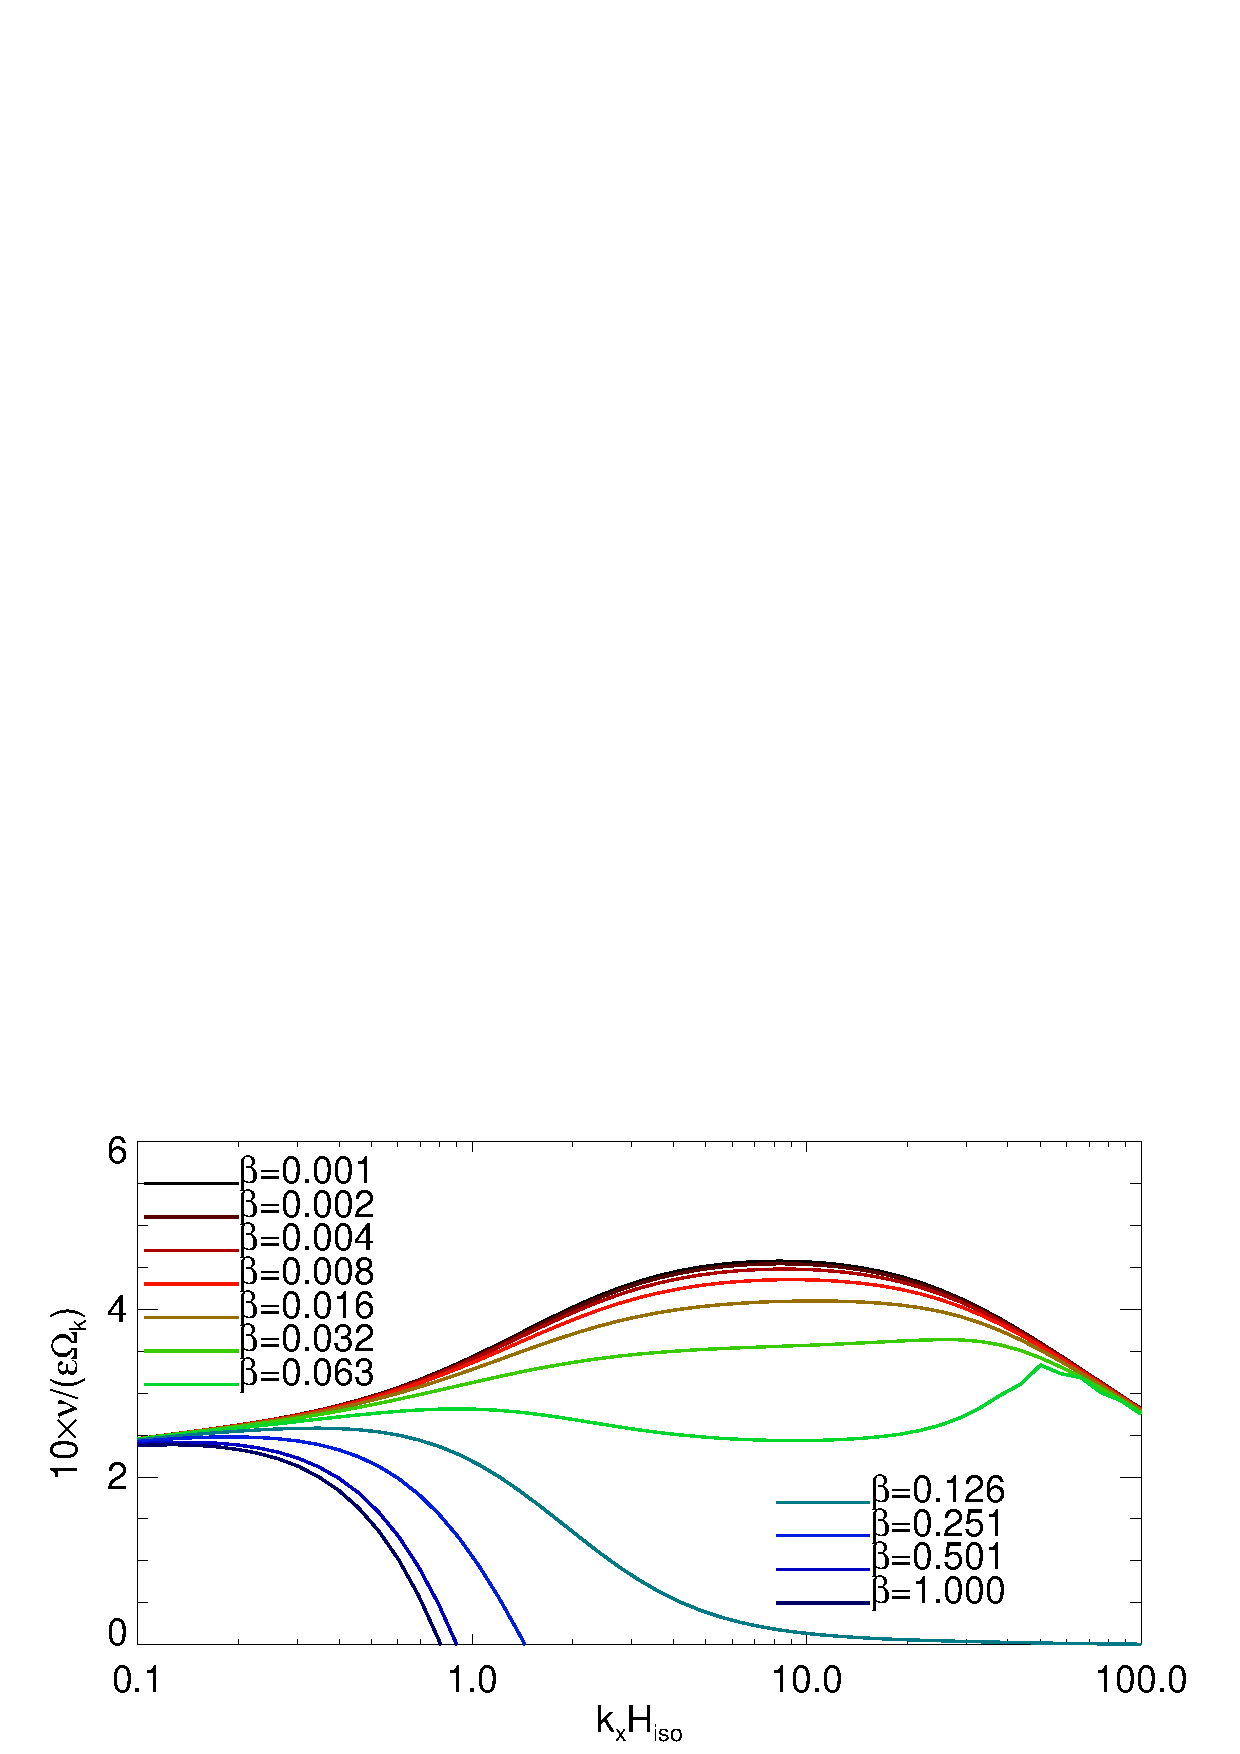
\includegraphics[width=\linewidth,clip=true,trim=0cm 0.0cm 0cm
%    0cm]{figures/compare_eigen_imag_bloop} 
%   % 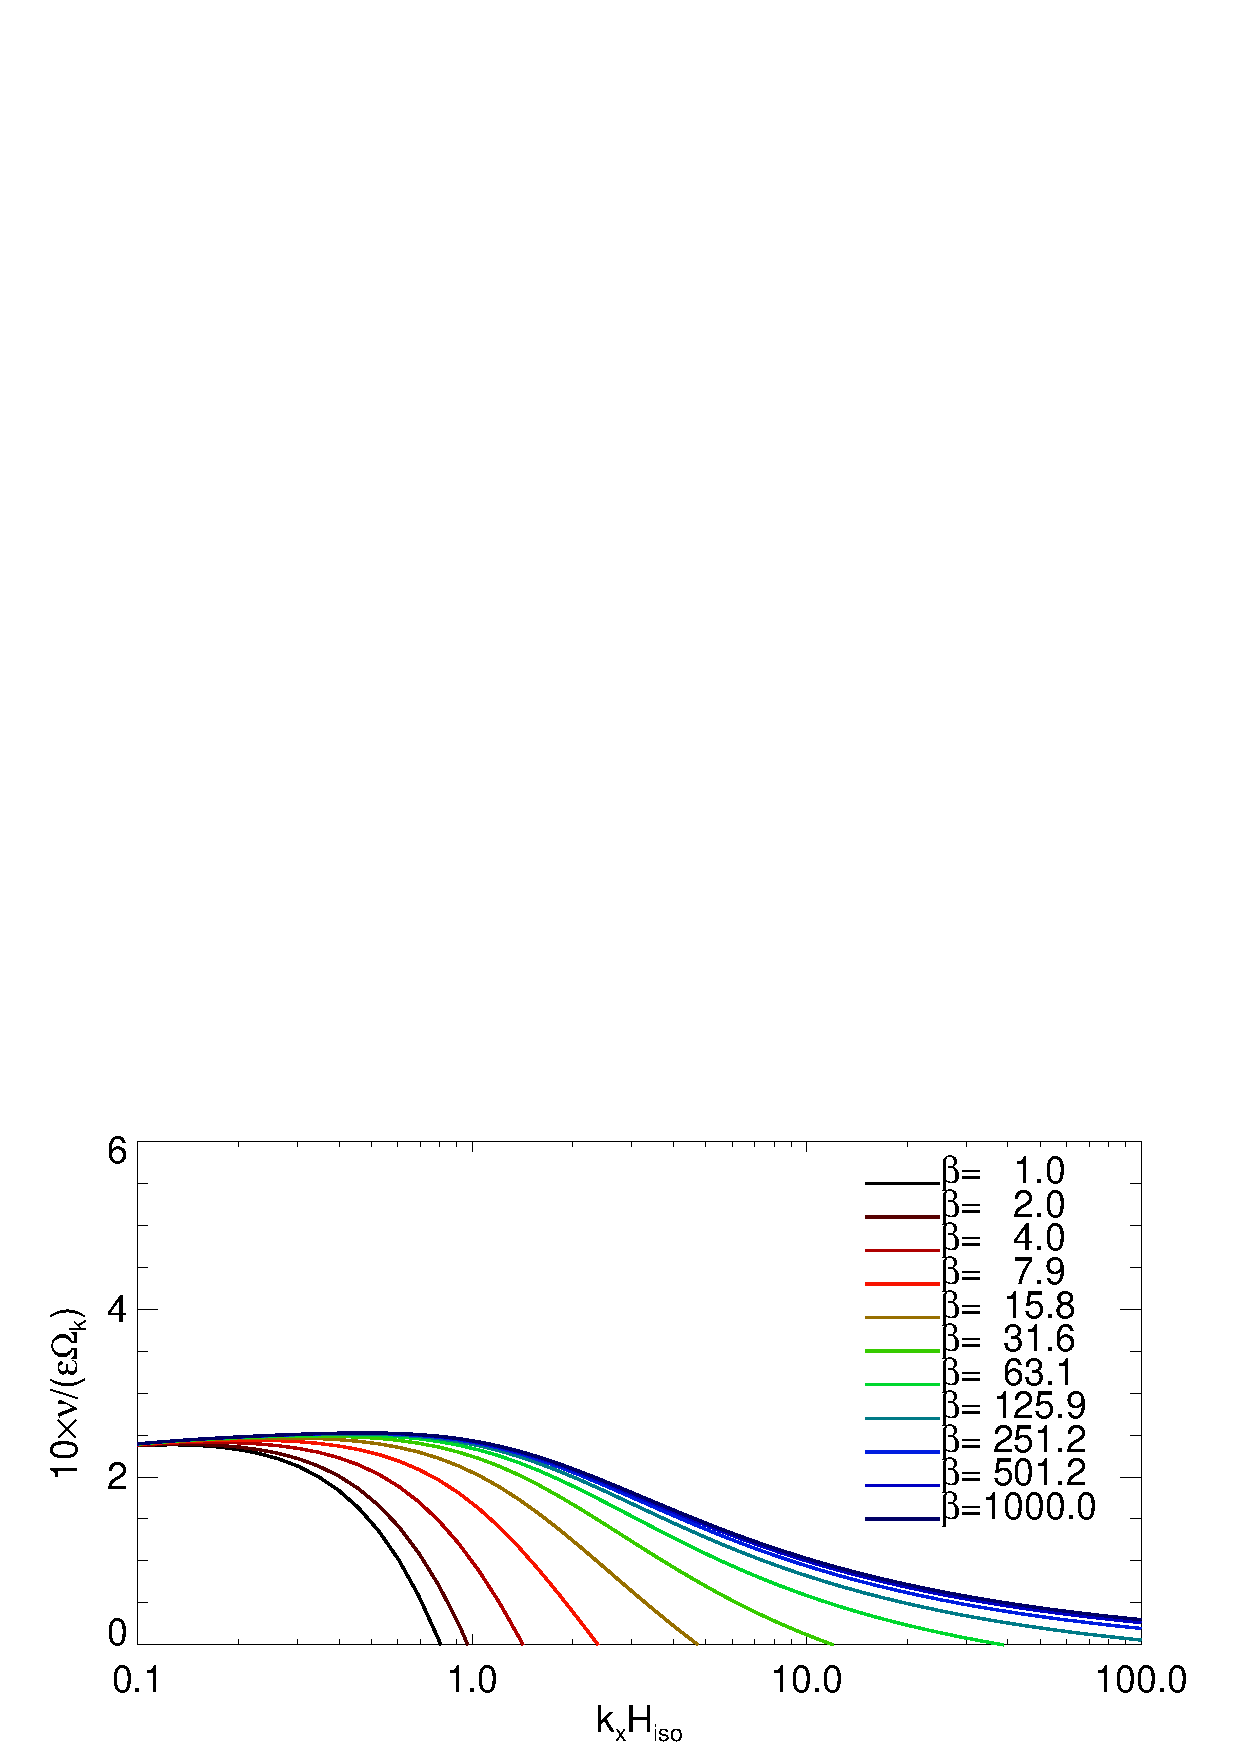
\includegraphics[width=\linewidth,clip=true,trim=0cm 0cm 0cm
%   % 1cm]{figures/compare_eigen_imag_bloop2} 
%   \caption{Growth rates of the fundamental VSI mode in 
%     nearly-vertically isothermal disks ($\Gamma=1.011$) with
%     $(p,q,\epsilon)=(-1.5,-1,0.05)$, evolved with $\gamma=1.4$ under a
%     range of thermal relaxation timescales   
%     $\beta$. The eigenfrequencies are calculated by numerically 
%     solving the full linear eigenvalue problem. \label{relax_growth_num}}   
% \end{figure} 

We visualize the effect of thermal relaxation in 
Fig. \ref{relax_eigenW_num} by comparing the eigenfunction $W$ for
$\beta=0.01$ and $\beta=0.1$. The latter value is close to the
critical value beyond which the fundamental VSI is stabilized
(\S\ref{iso_vsi_beta_crit}). Increasing $\beta$ 
restricts  the region in which $W\sim z$ closer to the midplane, with
oscillatory behavior emerging at the boundaries, where buoyancy first
becomes important. Finite thermal relaxation increases $|W|$ near the
vertical boundaries relative to that about the midplane, but
perturbations near the disk surface is unlikely important in practice
because the disk atmosphere contains little mass. 

% We also find this trend for fixed $\beta$ but
% increasing 
% $\khat$.  

\begin{figure}
  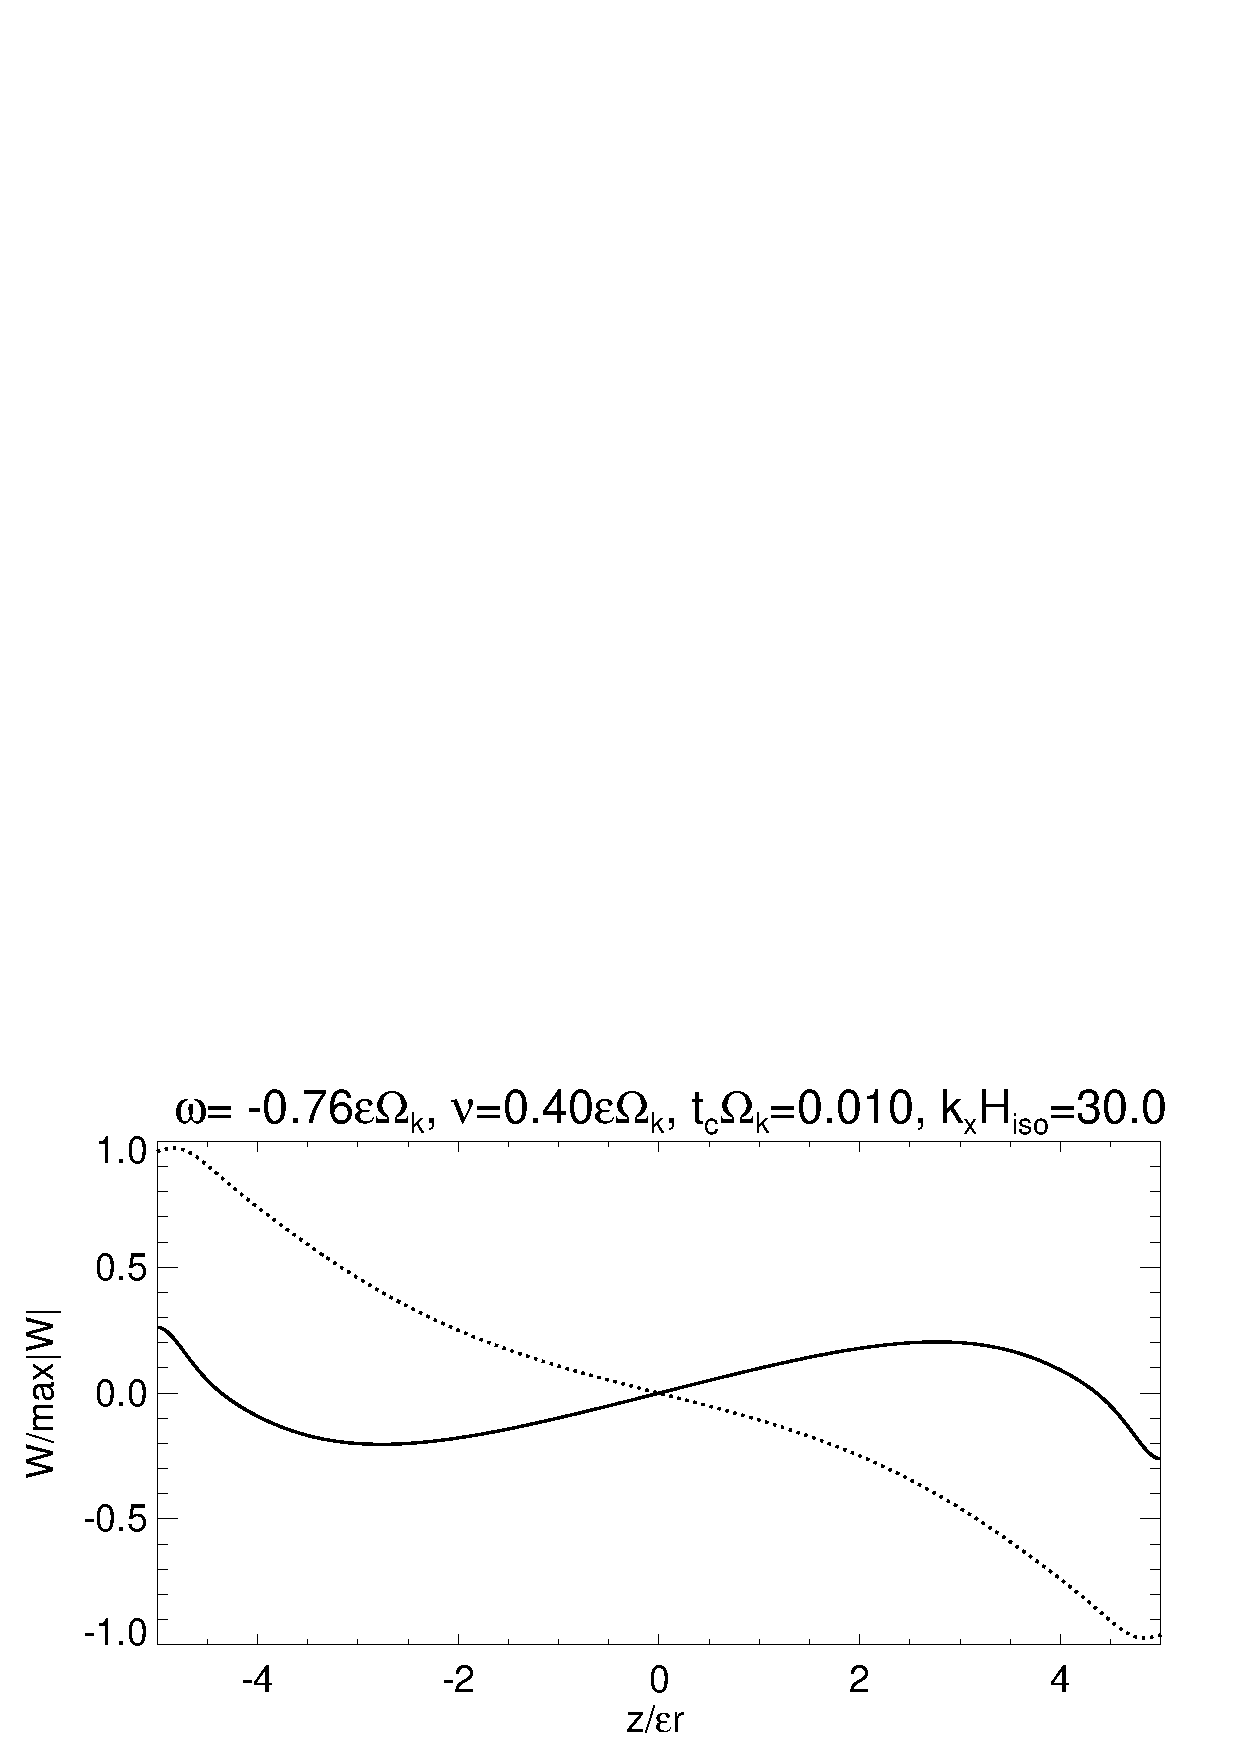
\includegraphics[width=\linewidth,clip=true,trim=0cm 1.75cm 0cm
  0cm]{figures/eigenvectorW_beta0d01} 
  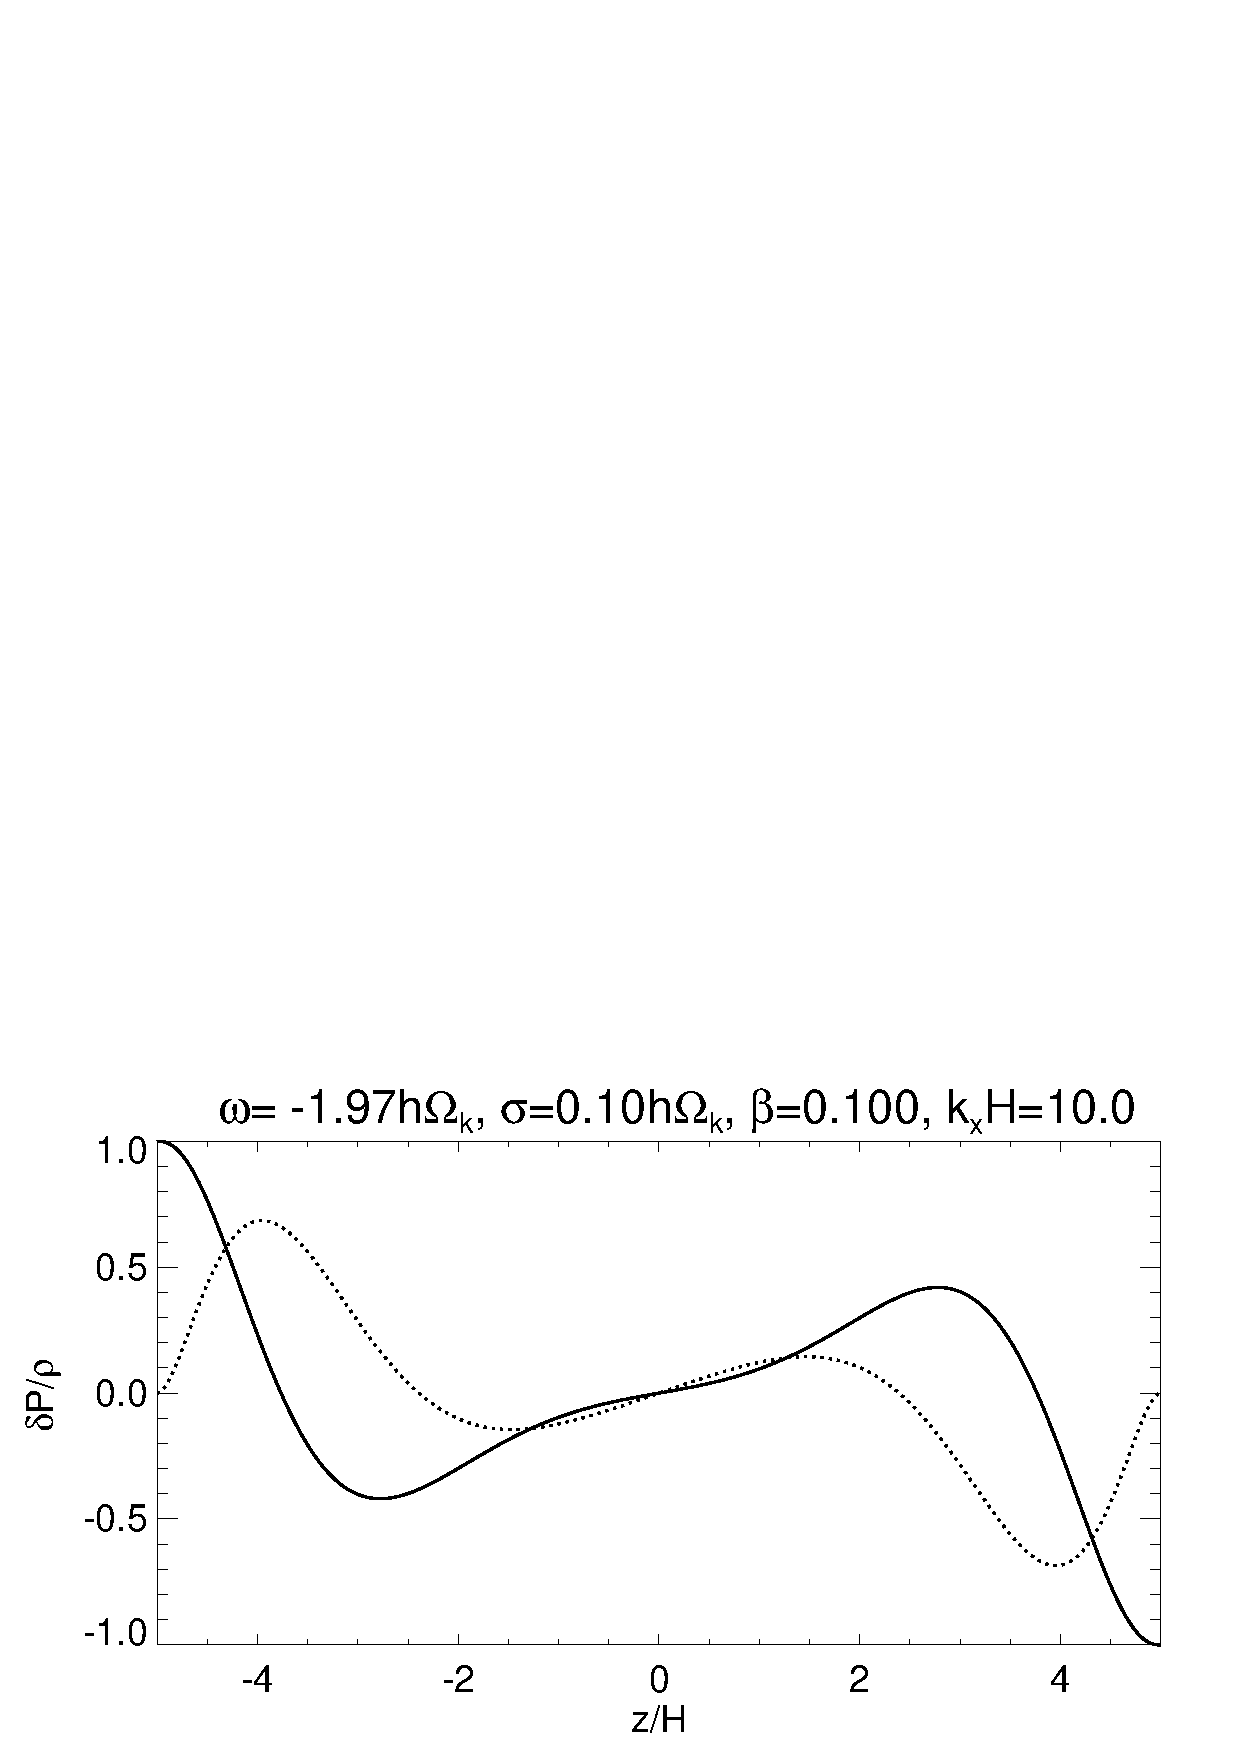
\includegraphics[width=\linewidth,clip=true,trim=0cm 0cm 0cm
  0cm]{figures/eigenvectorW_beta0d1} 
  \caption{Numerically-calculated eigenfunction of the fundamental VSI
    mode in a nearly vertically isothermal disk ($\Gamma=1.011$) with
    $(p,q,\epsilon)=(-1.5,-1,0.05)$, evolved with $\gamma=1.4$ and a dimensionless 
    thermal relaxation timescale $\beta \equiv t_c\Omega_k = 0.01$
    (top) and $0.1$ (bottom). The
    perturbation radial wavenumber is $\khat=30$. The
    real (imaginary) part of $W$ is plotted as the solid (dotted)
    line.
    \label{relax_eigenW_num}}  
\end{figure}

\subsection{Critical thermal relaxation timescale}
% may need to explain why choose k=10
% bcrit independent of k for k>>1 
% for some parameter regimes (e.g. large q, large epsilon) 
% behavior at larger kx and finite bcool not understood. 
We test our estimate for the maximum thermal relaxation timescale 
$\beta_\mathrm{crit}$ for the fundamental
VSI (Eq. \ref{iso_vsi_cond}). We use the previous disk
parameters as a reference point and vary $q\in[-0.2,-1.2]$,
$\gamma\in[1.2,2.0]$, and $\epsilon\in[0.02,0.1]$
separately. 

Here we use a wavenumber $\khat=10$. 

% , in which case we find $\nu$
% changes sign as $\beta$ is increased from zero. We find that with
% $\khat=30$, as used in the previous section, when $\beta$ is not small $\nu$ did not reach zero but instead decreases
% rapidly after the expected value of $\beta_\mathrm{crit}$.  These
% modes were found to have large amplitudes near the boundaries.  



%we suspect boundary conditions may play a role for 

% For large $\khat$ \emph{and} finite
% thermal relaxation (e.g. $\khat=30$, $\beta\gtrsim 0.2$) we found
% $\nu$ did not reach zero, but still decreases rapidly after the
% expected $\beta_\mathrm{crit}$. These modes have large perturbations
% near the boundaries, which may play a role not accounted for in our
% analytical discussion.  


The numerically-obtained $\beta_\mathrm{crit}$ is shown in
Fig. \ref{bcrit_compare} in comparison with Eq. \ref{iso_vsi_cond}.  

Our numerical results generally agree with 
Eq. \ref{iso_vsi_cond}. The agreement improves with decreasing  $|q|$,
$\epsilon$ and increasing $\gamma$, i.e. weaker instability. 
There is a noticeable difference as $\gamma\to1$ because the
derivation of $\beta_\mathrm{crit}$ assumed $\gamma>1$.  

\begin{figure}
  \includegraphics[width=\linewidth,clip=true,trim=0cm 0.cm 0cm
  0cm]{figures/bcrit_compare_q.ps} 
  \includegraphics[width=\linewidth,clip=true,trim=0cm 0.0cm 0cm
  0.8cm]{figures/bcrit_compare_g.ps}
  \includegraphics[width=\linewidth,clip=true,trim=0cm 0.0cm 0cm
  0.8cm]{figures/bcrit_compare_e.ps} 
  \caption{Dependence of the upper limit to the thermal relaxation timescale
    $\beta_\mathrm{crit}$ for the fundamental VSI mode on disk
    parameters. The fiducial parameters are $\Gamma=1.011$,
    $\gamma=1.4$ and $(p,q,\epsilon)=(-1.5,-1,0.05)$. Top: varying
    $q\in[-1.2,-0.2]$; middle: varying $\gamma\in[1.2,2.0]$; bottom:
    varying $\epsilon\in[0.02,0.1]$. The perturbation wavenumber is
    $\khat=10$. 
    \label{bcrit_compare}}  
\end{figure}


\subsection{Vertically non-isothermal disks}
We briefly consider vertically non-isothermal disks with 
$\Gamma=1.4$ and $(p,q,\epsilon)=(0,-1,0.05)$ as simulated in
\cite{nelson13}. In this case we set $\zmax\simeq2.2\epsilon r$, which
is close to the zero-density surface.     

% \subsubsection{$\gamma=\Gamma \neq 1$, $N_z^2\equiv 0$}
% Consider first the case $\gamma=1.4$ so that there is no vertical
% entropy gradient. We plot in Fig. the growth rates for the
% fundamental VSI for $\beta\in[10^{-2},10^{2}]$. We find growth rates
% do not reach zero, implying instability regardless of the thermal
% relaxation timescale if $\gamma=\Gamma$. This result is consistent
% with \cite{nelson13}.  Note that for $\beta\to\infty$ (adiabatic
% perturbations) and $\gamma=\Gamma$, the disk can be unstable according
% to the Solberg-Hoiland criterion  Eq. \ref{solberg2}.

% Growth rates for $\beta = 10^{-2}$ and
% $\beta=10^{2}$ behave similarly. This is not surprising because
% the linearized energy equation (Eq. \ref{lin_energy}) implies that 
% \begin{align}
%   W = \frac{\left(\Gamma^{-1} -
%       \ii\hat{\sigma}\beta\right)}{\left(1-\ii\hat{\sigma}\beta\right)}
%   Q \text{ for } \gamma\equiv \Gamma.   
% \end{align}
% Thus, $W \to Q/\Gamma$ as $\beta\to0$ and $W\to Q$ as
% $\beta\to\infty$. Since $\Gamma=O(1)$, these two limits are expected
% to produce qualitatively similar results. Interestingly,
% Fig. \ref{growth_vnoniso1} show that growth rates 
% maximize for $\beta=O(1)$. However, all growth rates are similar to
% order-of-magnitude for $0.1\lesssim\khat\lesssim 100$. 

% \begin{figure}
%   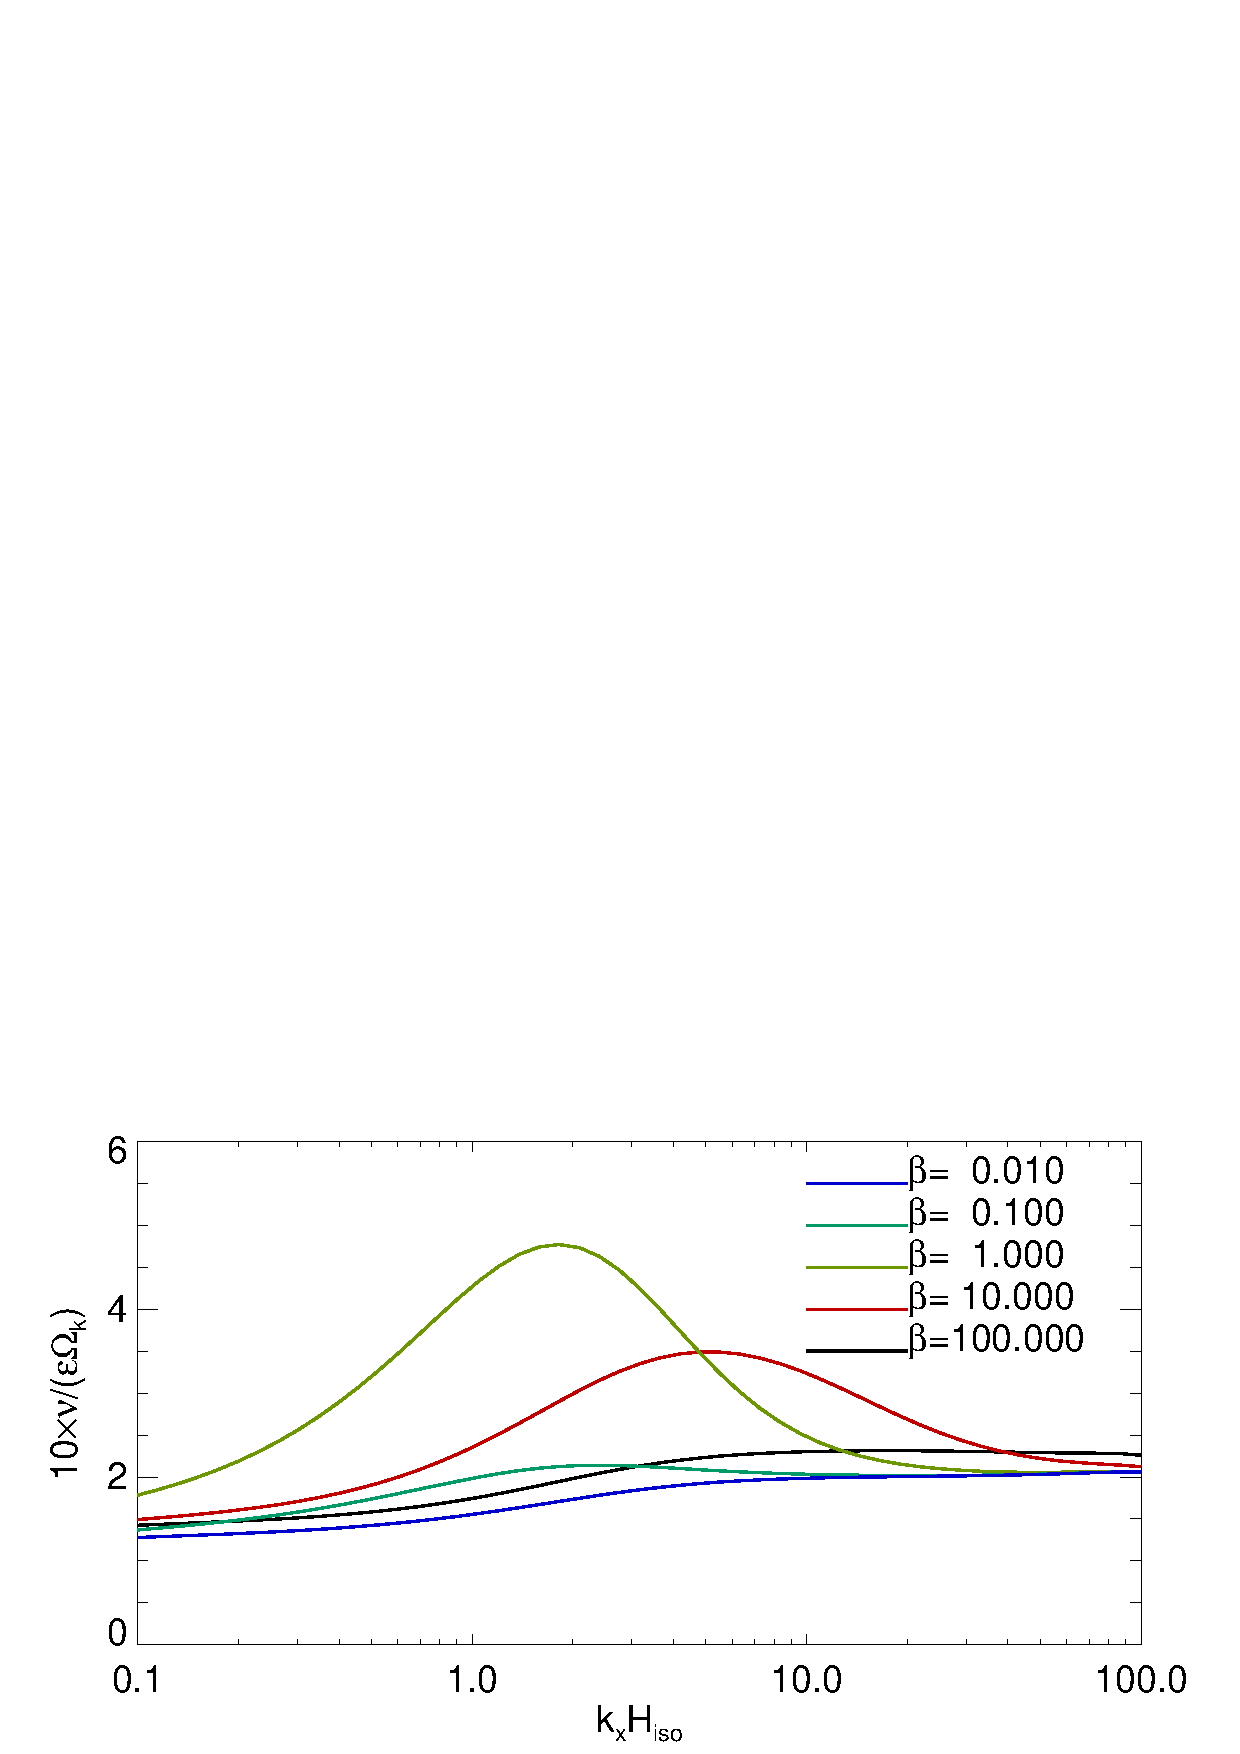
\includegraphics[width=\linewidth,clip=true,trim=0cm 0cm 0cm
%   0cm]{figures/growth_vnoniso1} 
%   \caption{Numerically-determined growth rates of the fundamental VSI
%     mode in neutrally-buoyant ($N_z^2\equiv0$), vertically non-isothermal disks
%     ($\Gamma=\gamma=1.4$), with $(p,q,\epsilon)=(0,-1,0.05)$, for
%     a range of thermal relaxation timescales 
%     $\beta$. \label{growth_vnoniso1}}     
% \end{figure} 

% \subsubsection{$\gamma\neq\Gamma \neq 1$, $N_z^2\geq0$}
% %gamma = 2.0, Gamma = 1.4, vary bcool 
% Finally, we introduce buoyancy in a vertically non-isothermal disk by
% setting $\gamma=2$. This scenario was not considered by  
% \cite{nelson13}, but is similar in spirit with vertically isothermal 
% disks evolved with $\gamma>1$, as considered in the previous section. 
% Fig. \ref{growth_vnoniso2} plots the fundamental VSI growth rates for
% this case. We observe the same trend as for vertically isothermal
% disks with $N_z^2\geq 0$ (Fig. \ref{relax_growth_num}), namely growth
% rates reach zero at finite $\khat$. From Fig.\ref{growth_vnoniso2} we
% expect the VSI to be strongly stabilized even for small, finite
% thermal relaxation times.  

% \begin{figure}
%   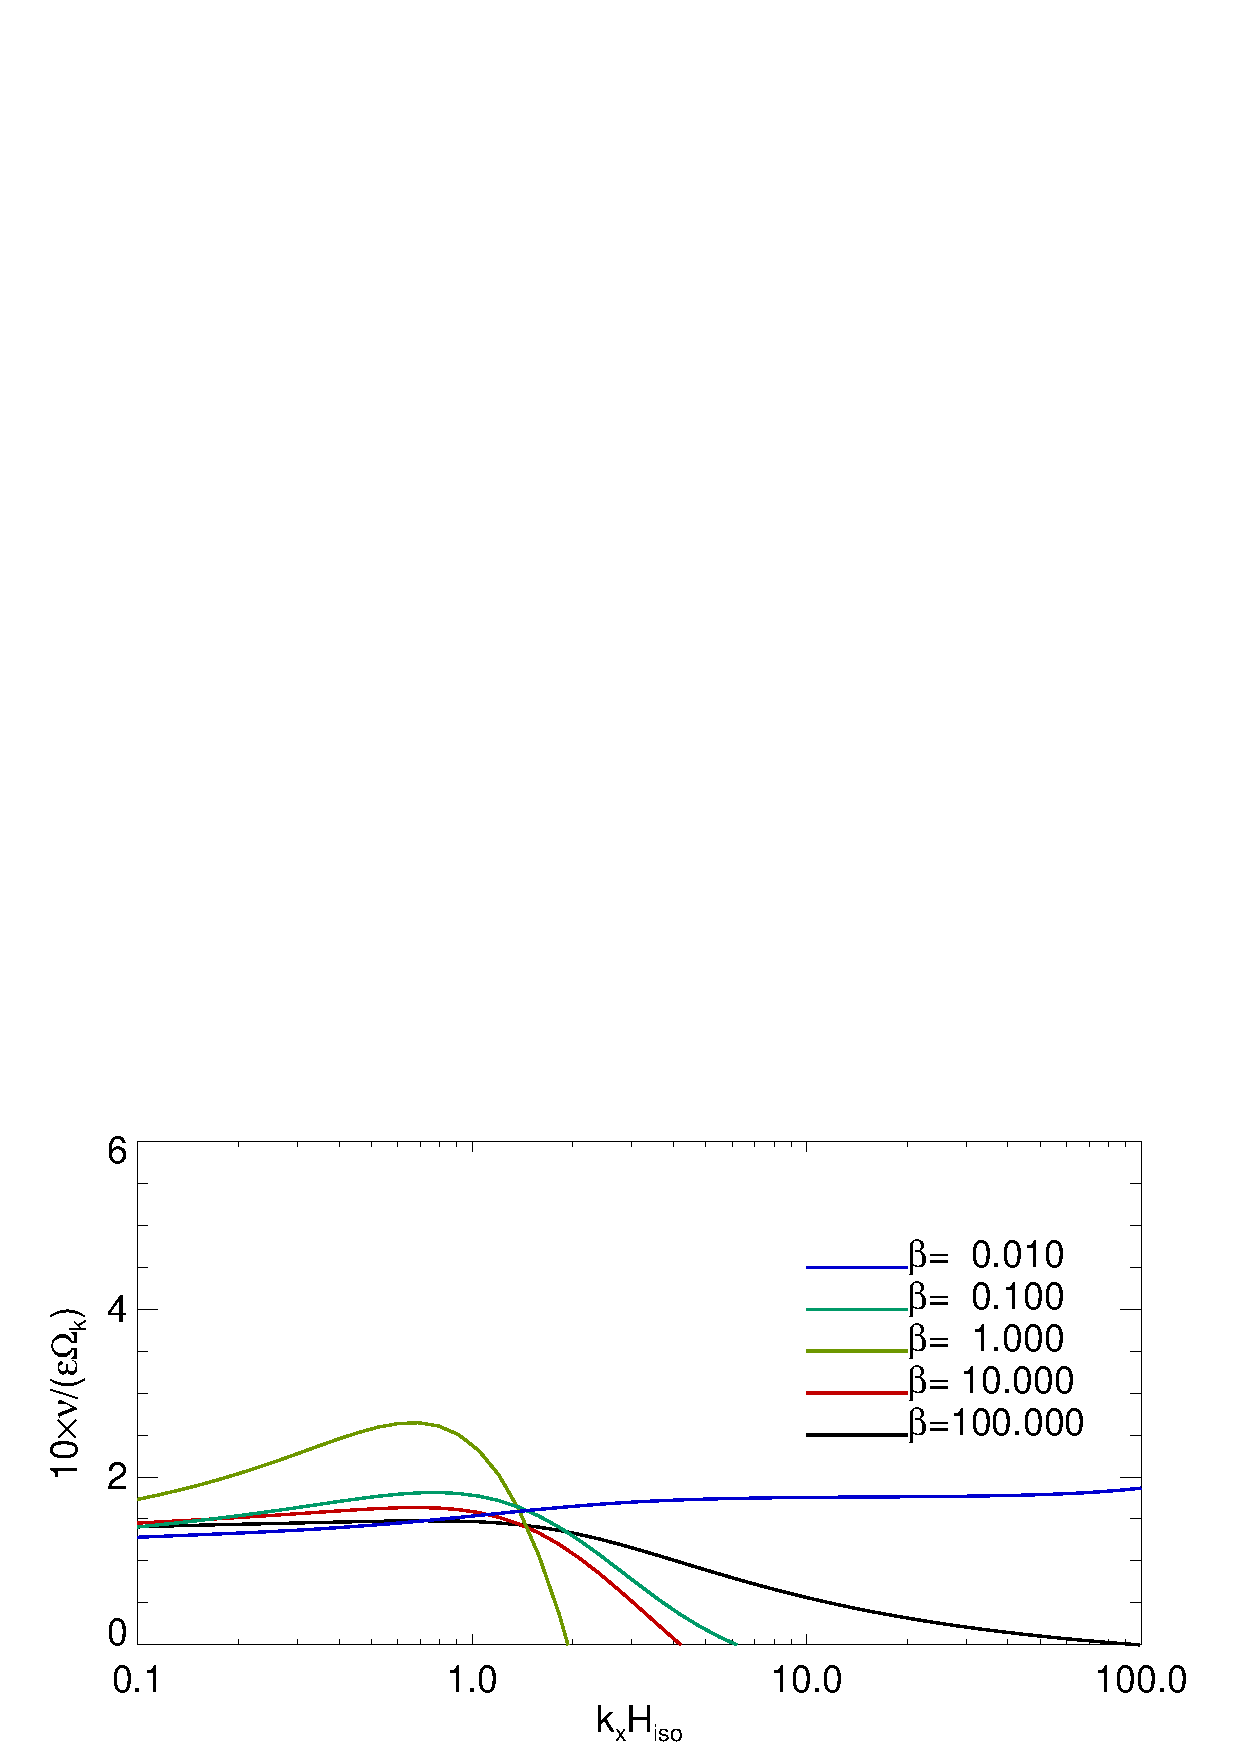
\includegraphics[width=\linewidth,clip=true,trim=0cm 0cm 0cm
%   0cm]{figures/growth_vnoniso2}
%   \caption{Same as Fig. \ref{growth_vnoniso1}, but with $\gamma=2$ so that
%     $N_z^2\geq0$. \label{growth_vnoniso2}}
% \end{figure} 

 





















% \subsection{VSI in a stably stratified disk}
% We demonstrate the (strong) stabilizing effect of a  
% positive vertical entropy gradient ($N_z^2\geq0$) by setting $\gamma=2$.  
% Since we expect the perturbations to decay rapidly
% away from the midplane (see \S\ref{analytic_adia}), we consider a
% smaller domain with $\zmax = 2\epsilon r$. 
% Other disk and perturbation parameters are the same as in
% \S\ref{vertiso_pertiso}.    

% Fig. \ref{lowfreq_eigen_adia} show the eigenvalues for this
% problem. The growth rates are much smaller than
% those in the previous section. The fundamental VSI mode is that with
% $\mathrm{max}\nu$. Its expected and numerically-calculated growth
% rates compares well, with 
% \begin{align*}
%   \nu = 0.03751 \epsilon \Omega_k &\quad \text{(from
%     Eq. \ref{gam2_growth_rate})},\\
%   \nu = 0.03672 \epsilon \Omega_k &\quad \text{(numerical)}.
% \end{align*}
% The fundamental mode is plotted in Fig. \ref{lowfreq_eigenfunc_adia},
% and clearly show that perturbations are rapidly stabilized away from
% the midplane. For the adopted disk and perturbation parameters,
% Eq. \ref{gam2_alpha} gives $\real{\alpha}\simeq - 43.8$, corresponding
% to a characteristic decay length scale of $\sqrt{2/|\alpha|}\epsilon r\simeq 0.2\epsilon r$,
% which is consistent with that observed in  Fig. \ref{lowfreq_eigenfunc_adia}. 

% This decay lengthscale is rougly the height within which
% vertical shear is larger than the buoyancy frequency squared. That is,
% \begin{align*}
% \left|r\frac{d\Omega^2}{dz}\right|\gtrsim N_z^2
% \end{align*}
% for
% \begin{align*}
%   \left|\frac{z}{\epsilon r}\right| \lesssim \frac{\epsilon|q|\gamma}{\gamma-1},
% \end{align*}
% in a thin, vertically isothermal disk. This evaluates to $|z|\lesssim
% 0.2\epsilon r$ for the current disk model, consistent with
% Fig. \ref{lowfreq_eigenfunc_adia}. 

% Furthermore, the growth rate to should be no larger than the
% maximum vertical shear available within this decay lengthscale. Using 
% Eq. \ref{max_growth} as a rough guide, 
% \begin{align}
%   \frac{\nu}{\epsilon\Omega_k}<\frac{\epsilon |q|^2\gamma}{2(\gamma-1)},
% \end{align}
% or $\nu< 0.1\epsilon\Omega_k$ in our disk model,
% consistent with numerical results. 

% \begin{figure}
%   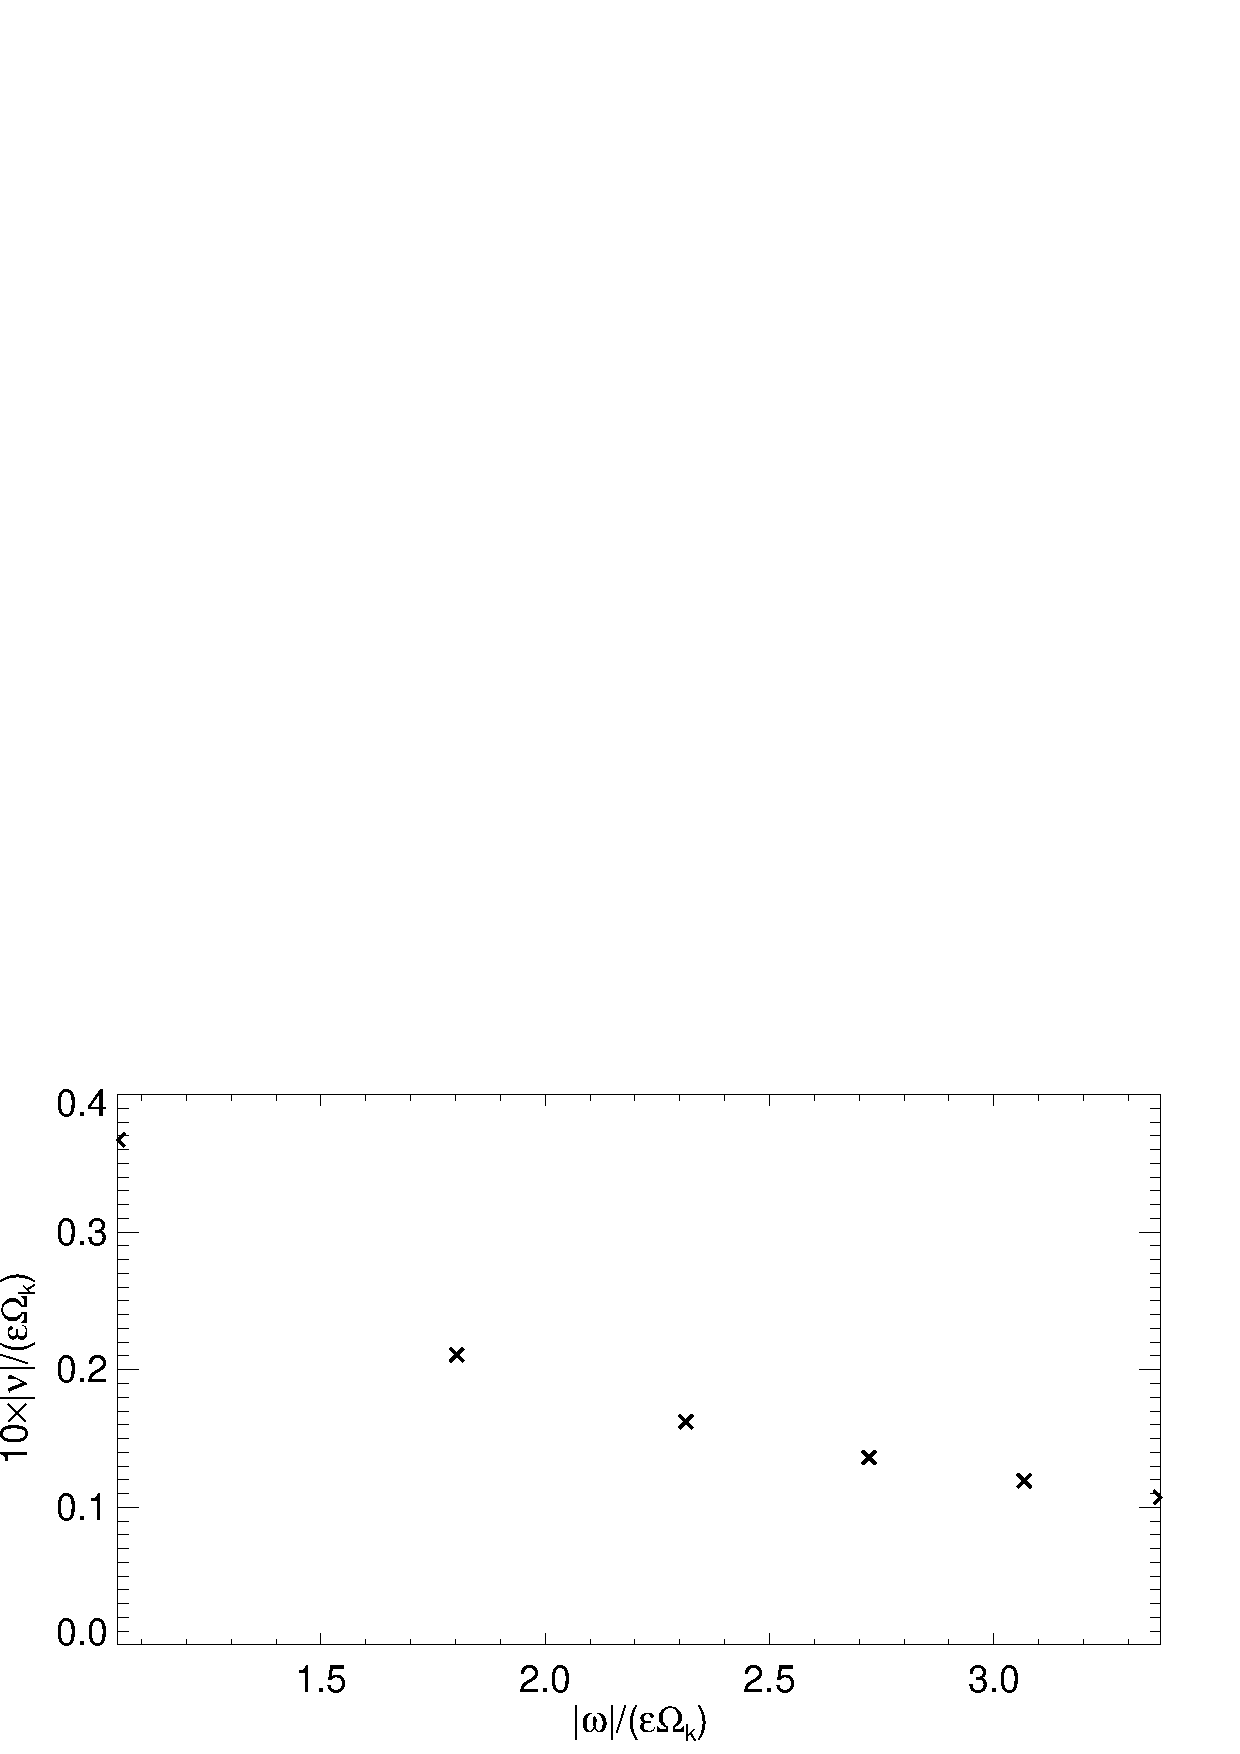
\includegraphics[width=\linewidth]{figures/eigenvalues_adia}
%   \caption{Eigenvalues in for the
%     VSI in a nearly vertically isothermal disk
%     ($\Gamma=1.011$) with $(p,q,\epsilon)=(-1.5,-1,0.1)$, 
%     evolved adiabatically with $\gamma=2$. The perturbation radial
%     wavenumber is $\khat=20\pi$. \label{lowfreq_eigen_adia}
%   }
% \end{figure}
  

% \begin{figure}
%   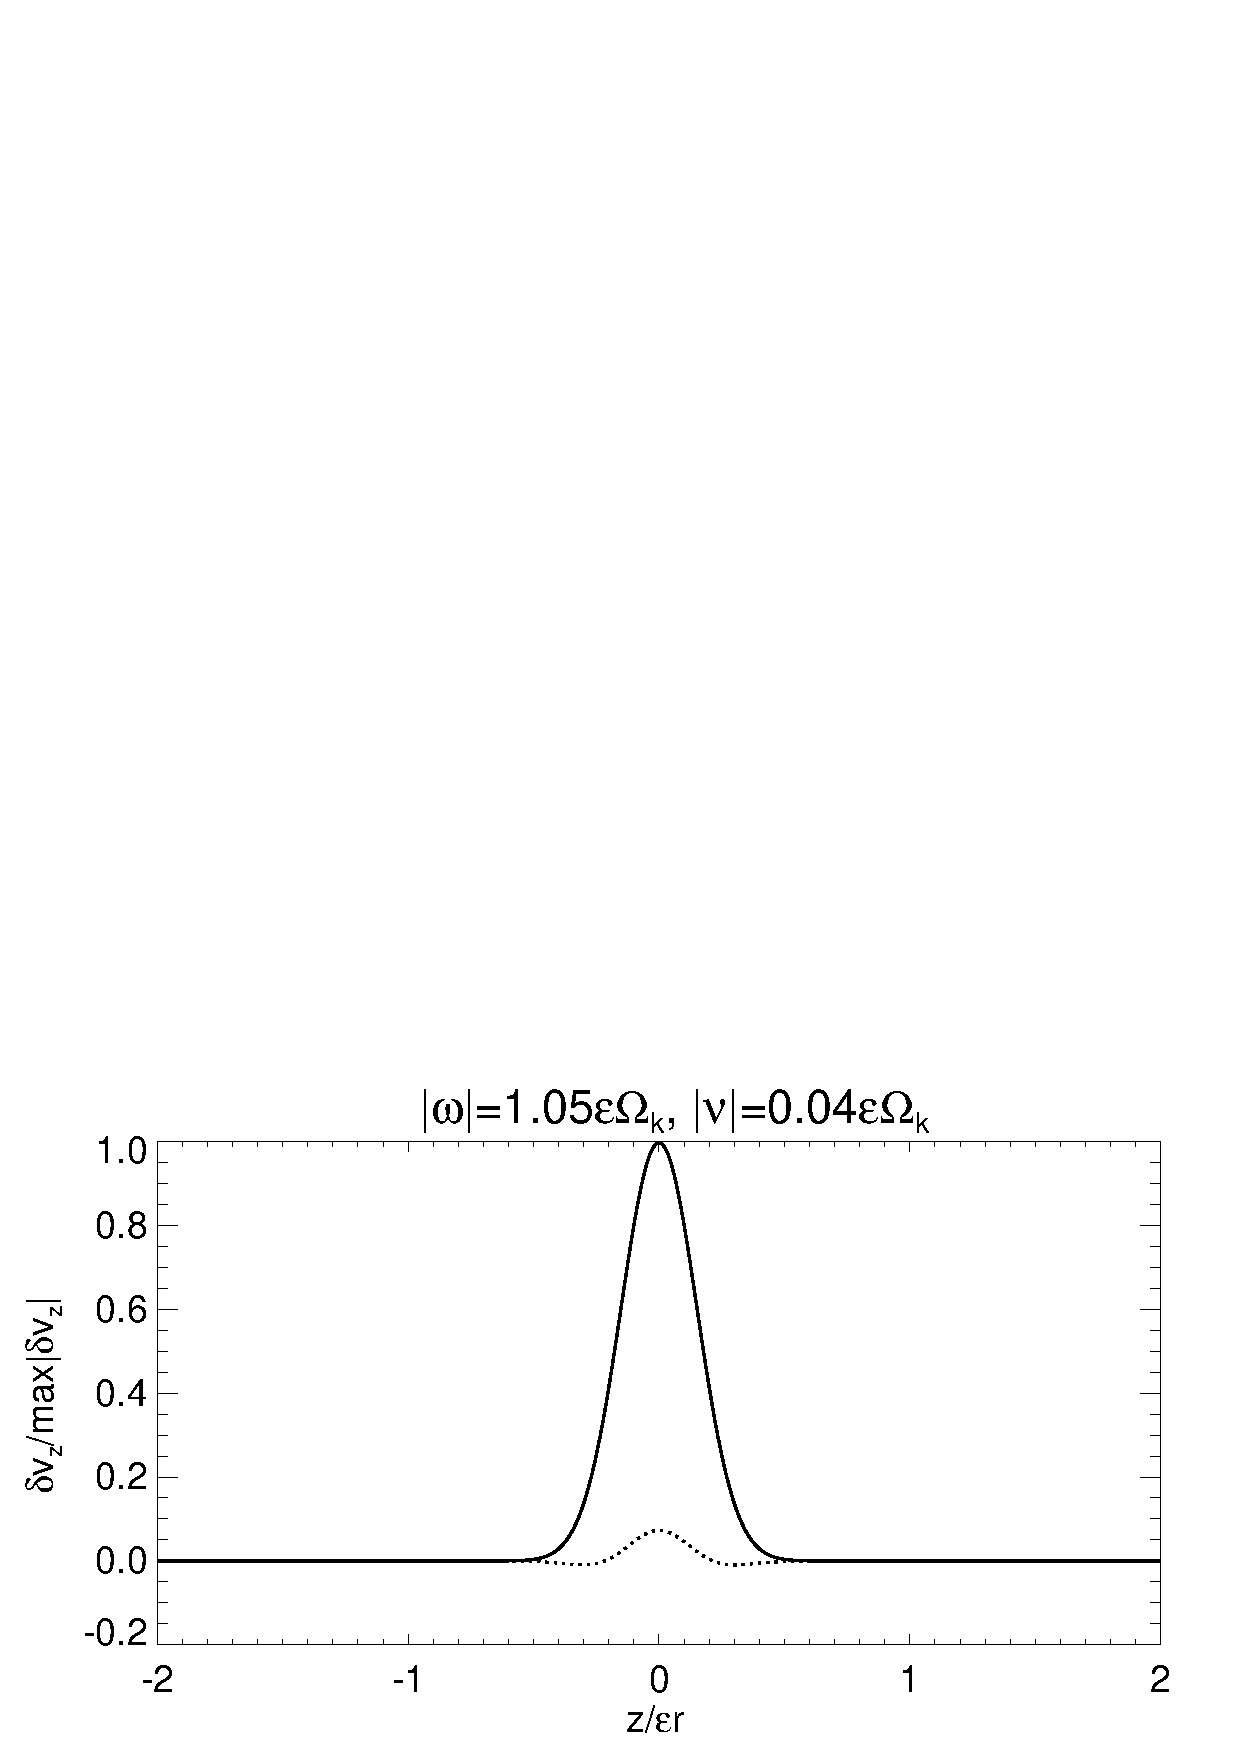
\includegraphics[width=\linewidth]{figures/eigenvectorvz_adia}
%   \caption{Fundamental VSI mode in a nearly vertically
%     isothermal disk ($\Gamma=1.011$) with $(p,q,\epsilon)=(-1.5,-1,0.1)$, 
%     evolved adiabatically
%     with $\gamma=2$. This eigenfunction 
%     corresponds to the top-left eigenvalue displayed in 
%     Fig. \ref{lowfreq_eigen_adia} (largest $|\nu|$).  
%     The  real (imaginary) part of $\delta v_z$ are shown as solid
%     (dotted) lines. 
%     \label{lowfreq_eigenfunc_adia}
%   }
% \end{figure}

% Although a positive vertical entropy gradient is stabilizing, we note
% that $N_z^2\propto z^2$  while vertical shear $rd\Omega^2/dz\propto
% z$, so that there is always a region sufficiently close to the
% midplane in which vertical shear dominates over bouyancy and the VSI
% can operate. However, the growth rates are small and the instability
% only affects the regions close the midplane. These modes may not be
% important in practice.  


% \subsection{Other adiabatic indices}
% To see the transition from neutrally-bouyant to stably stratified cases above, 
% we repeated the previous calculation with $\gamma\in[1,2]$. 
% We restore the vertical domain to $\zmax=10\epsilon r$. 
% Fig. \ref{adia_growth_num} shows the eigenfrequencies of the
% fundamental VSI mode. 


% %To select the appropriate
% %eigenvalues we vary the parameters slowly away from a reference solution.   
% % The numerically-determined eigenfrequencies are qualitatively
% % consistent with the discussion in \S\ref{adia_compare_gam1}.
% There is good agreement between Fig. \ref{adia_growth_num} and
% Fig. \ref{adia_growth} for $\khat=k_xH_\mathrm{iso}\gtrsim1$. There is a
% mismatch for smaller wavenumbers, especially in the growth
% rates. Actual growth rates decrease slower as $\khat\to0$
% than that in Fig. \ref{adia_growth}. Disagreement at small
% $\khat$ is not unexpected because the low-frequency
% approximation used to obtain Fig. \ref{adia_growth} becomes invalid since
% $|\omega|\sim\Omega_k$ for small $\khat$.  

% Given the number of approximations made in \S\ref{adia_compare_gam1},
% Fig. \ref{adia_growth_num} compares well with 
% Fig. \ref{adia_growth}. The main qualitative features of the full
% numerical solution in Fig. \ref{adia_growth_num} are captured by
% Fig. \ref{adia_growth}: stabilization for 
% $\khat\to0$ and $\khat\to\infty$,
% stabilization for increasing $\gamma$ (but ineffective at small $\khat$), 
% and the shift of the most unstable wavenumber to smaller values as
% $\gamma$ is increased. 


% \begin{figure}
%   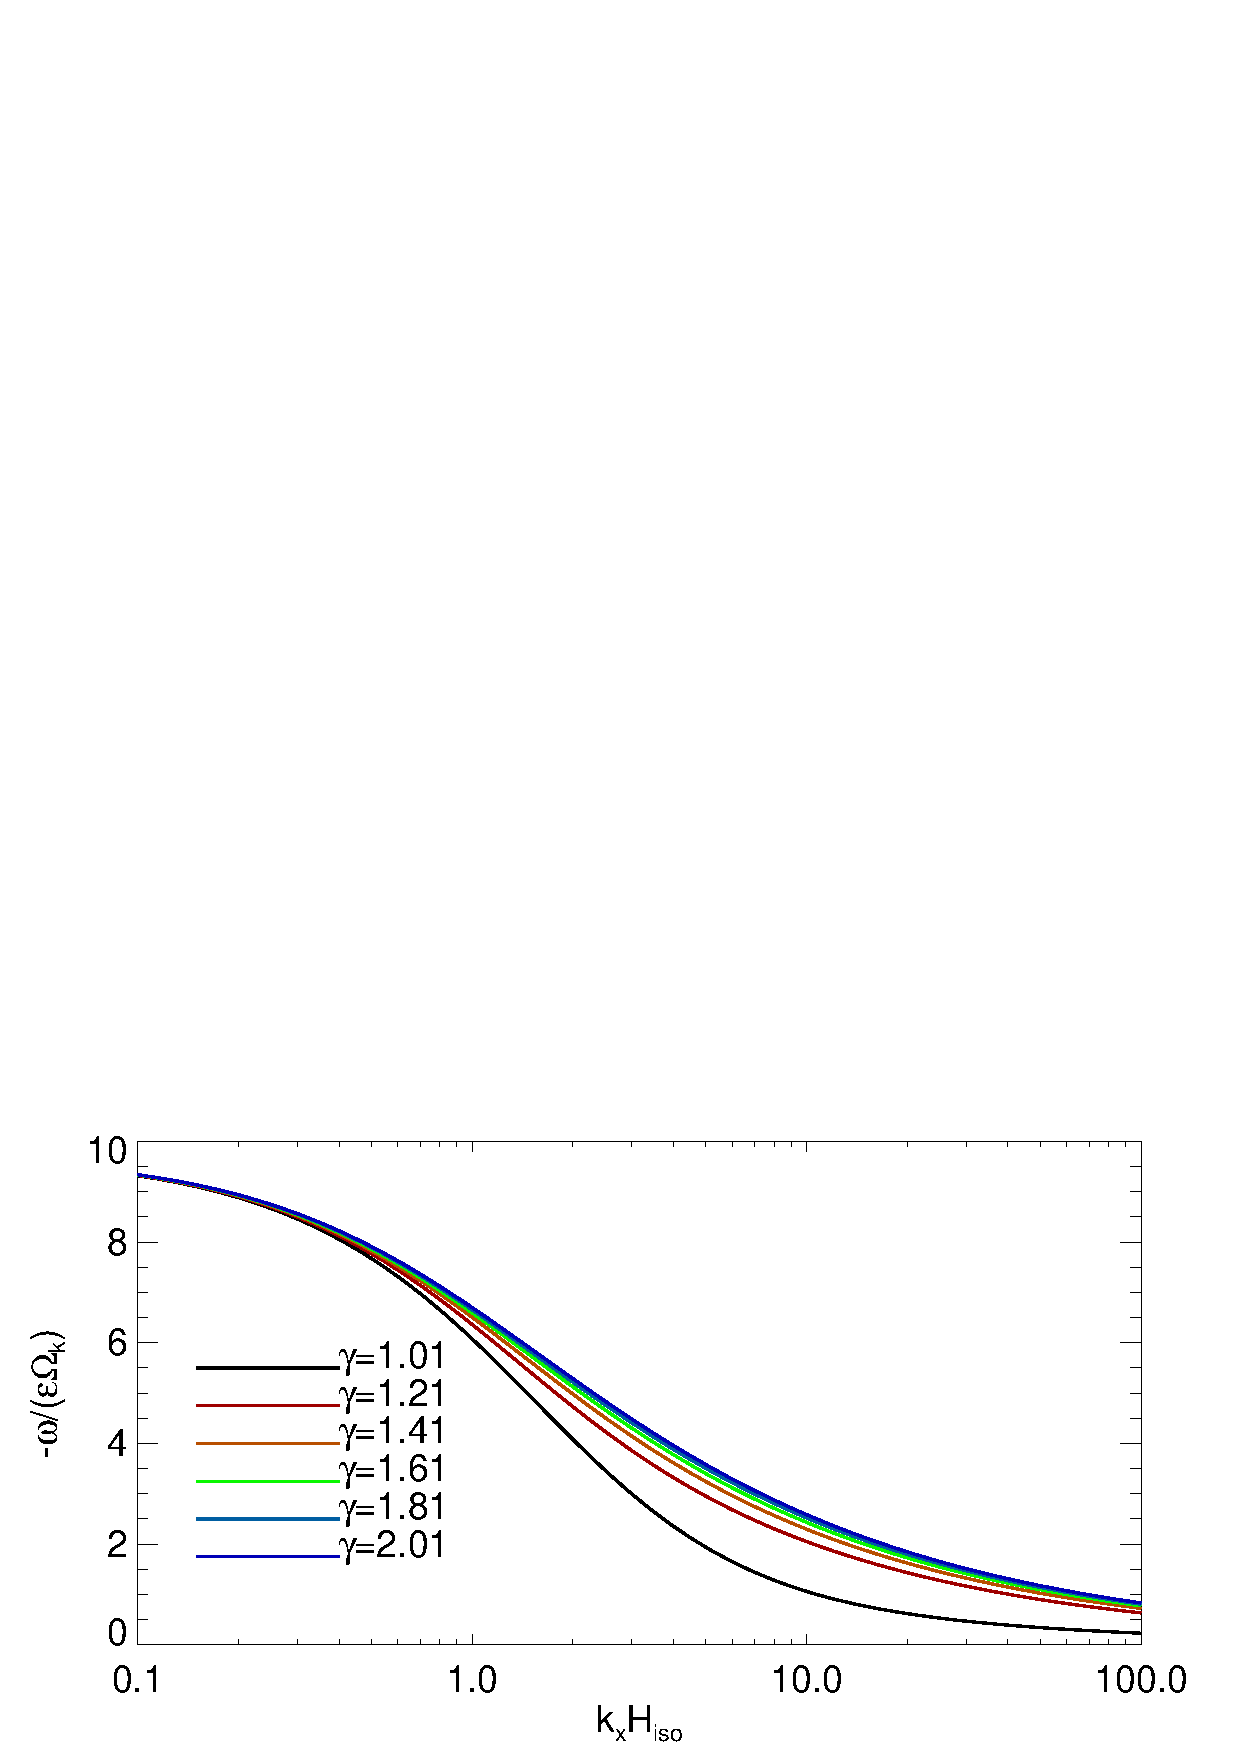
\includegraphics[width=\linewidth,clip=true,trim=0cm 1.75cm 0cm 0cm]{figures/compare_eigen_real1}
%   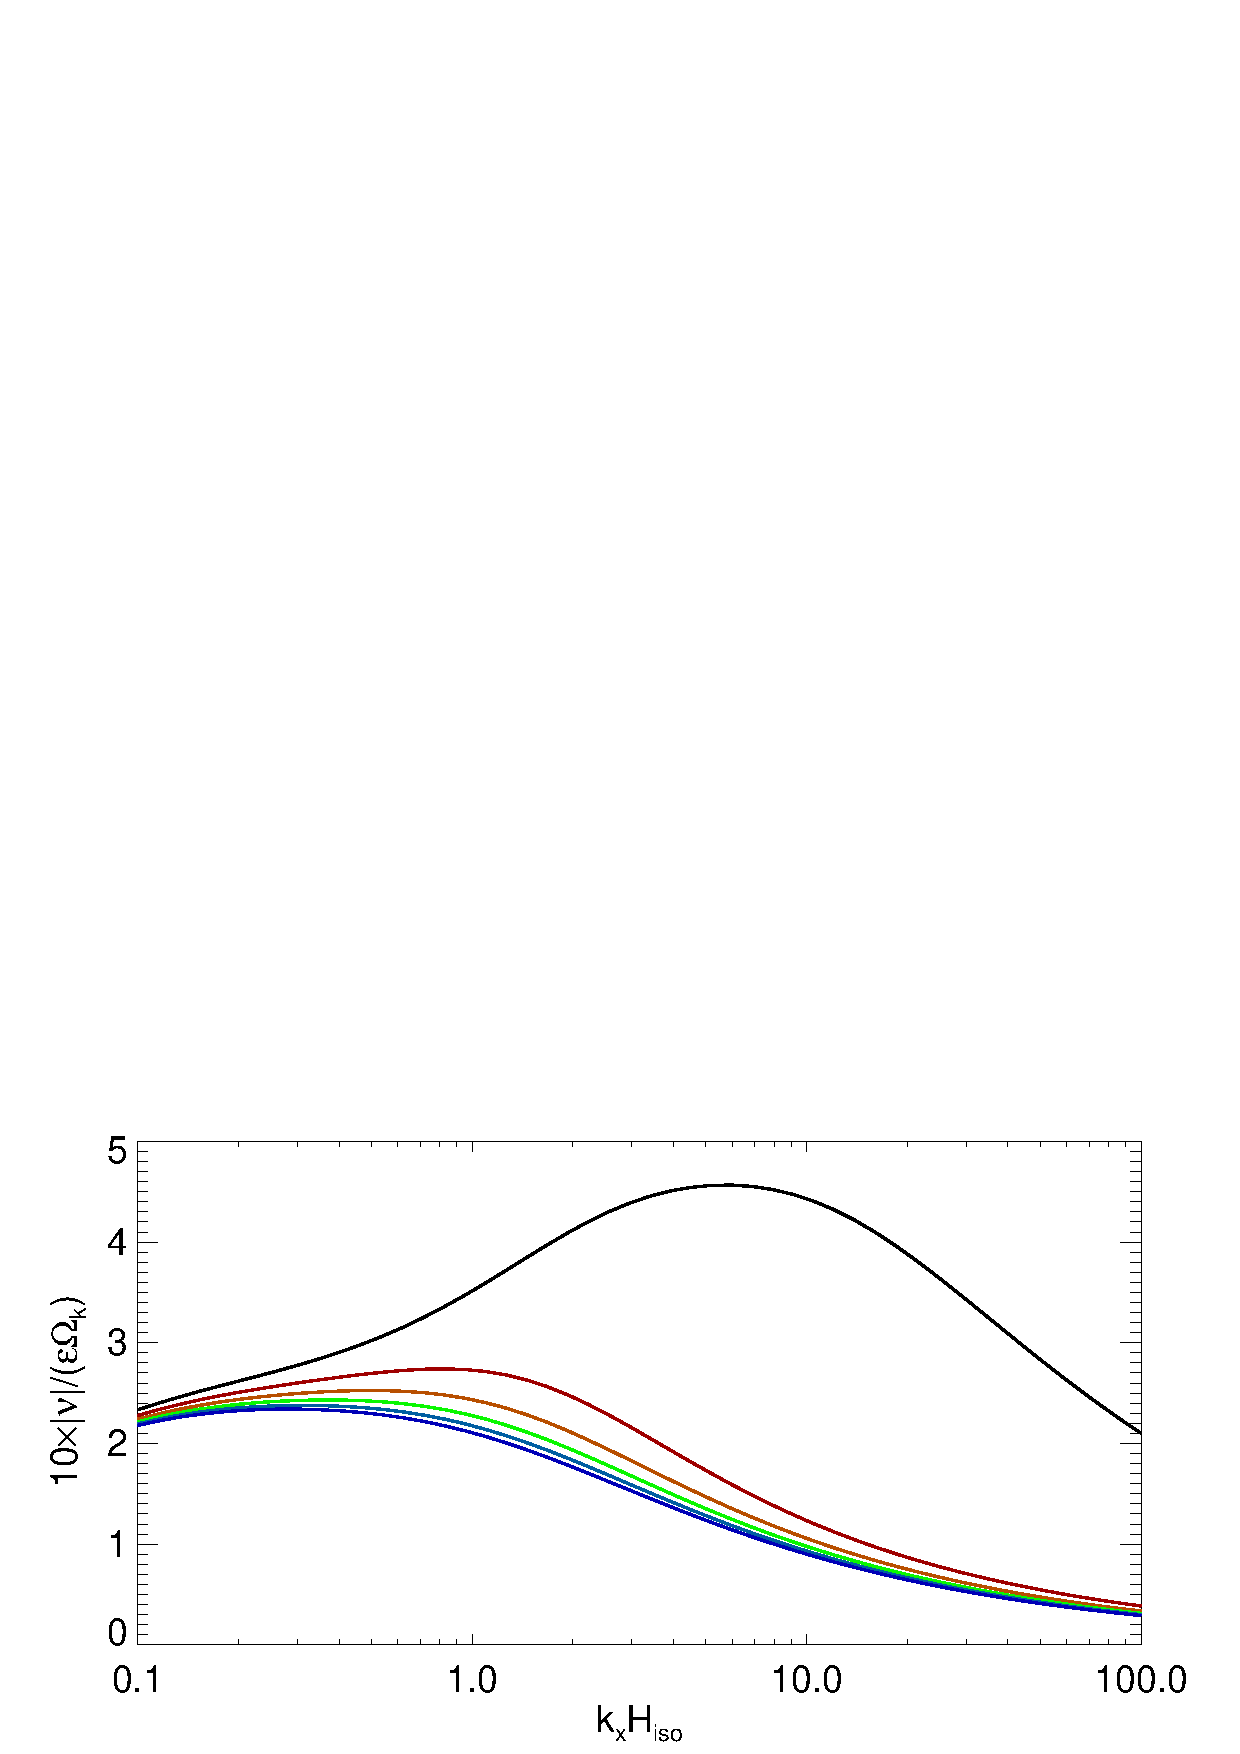
\includegraphics[width=\linewidth,clip=true,trim=0cm 0cm 0cm 1cm]{figures/compare_eigen_imag1}
%   \caption{Real frequency (top) and growth rate 
%     (bottom) of the fundamental VSI in a nearly vertically   
%     isothermal disks ($\Gamma=1.011$) with $(p,q,\epsilon)=(-1.5,-1,0.1)$, 
%     subject to adiabatic perturbations with different values of $\gamma$. 
%     The eigenfrequencies are calculated by numerically
%     solving the full linear eigenvalue problem. This plot is to
%     be compared with Fig. \ref{adia_growth}. \label{adia_growth_num}}   
% \end{figure}  
